\chapter{Diseño}
\label{chap:deseño}

\lettrine{E}{n} este capítulo se describe la organización interna de la aplicación y las principales decisiones de diseño adoptadas en sus tres subsistemas: backend, frontend y Android. El objetivo ha sido mantener una estructura coherente con el dominio funcional del proyecto, facilitar el mantenimiento del código y conservar una separación clara entre persistencia, lógica de negocio, exposición de servicios e interfaz de usuario.

\section{Introducción y objetivos}

El diseño parte de una idea principal: el sistema debe permitir coordinar emergencias, recursos y avisos de forma consistente, sin duplicar responsabilidades entre capas. Para ello, el backend concentra el modelo de dominio y las reglas de negocio, el frontend web actúa como interfaz de gestión principal y la aplicación Android adapta parte de esas funcionalidades a un contexto móvil, manteniendo el acceso a la información operativa y a las acciones más frecuentes.

En la evolución respecto al trabajo previo \cite{TFGAdrianGarcia2025} se han incorporado nuevas funcionalidades, especialmente en torno a las asignaciones, el envío de notificaciones y la generación de recomendaciones basadas en reglas. La estructura general de la interfaz y del dominio se mantiene porque el objetivo no era redefinir la aplicación completa sino ampliar su alcance funcional sobre una base ya establecida. Al existir una base escalable, se han podido añadir funcionalidades sin reestructurar completamente el sistema, si bien se han tenido que realizar modificaciones, aunque de menor complejidad de la que habría supuesto partir de un diseño completamente nuevo. 

\section{Resumen de patrones usados}
\label{sec:patrones}
Parte de la arquitectura y de las decisiones de diseño utilizadas en este proyecto han sido heredadas y adaptadas a partir del trabajo previo desarrollado. Esta reutilización no solo permite mantener una continuidad tecnológica, sino también reducir la complejidad de desarrollo al apoyarse en una base arquitectónica ya consolidada.

Entre los patrones heredados destaca especialmente la organización en capas, utilizada tanto en el backend como en el frontend, permitiendo separar claramente las responsabilidades de presentación, lógica de negocio y persistencia de datos. Esta división facilita el mantenimiento del código, mejora la modularidad y simplifica la evolución futura de la aplicación. Del mismo modo, se mantiene una estructura basada en el patrón Modelo-Vista-Controlador (MVC), especialmente en la parte de interfaz, favoreciendo una separación clara entre la representación visual, la gestión del estado y la interacción con el usuario.

También se utilizan mecanismos de abstracción y desacoplamiento como la inyección de dependencias, que facilita la reutilización de componentes y reduce el acoplamiento entre módulos, o el uso de objetos específicos para la transferencia de información entre capas, permitiendo encapsular y estructurar adecuadamente los datos intercambiados dentro del sistema. Además, se conservan patrones orientados al acceso y manipulación de datos, contribuyendo a aislar la lógica de persistencia del resto de la aplicación y mejorando la mantenibilidad general del proyecto.

Junto a estos patrones heredados, se han incorporado otros vinculados a la lógica de recomendación del backend y a la comunicación asíncrona y navegación de la aplicación Android. A continuación se resumen los principales patrones añadidos.

\begin{itemize}

    \item \textbf{API-first con OpenAPI:} En este proyecto se ha adoptado un diseño \textit{API-first}, definiendo primero el contrato de la API en un fichero YAML con OpenAPI y generando a partir de él las interfaces de controladores y los DTOs del backend mediante el plugin de Maven de OpenAPI. Gracias a esto se ha generado la documentación mediante Swagger de forma automática, lo que facilita la sincronización entre la implementación y la documentación y reduce errores de desalineación entre ambos. Este enfoque ha permitido que los contratos de la API se generen de forma consistente, lo que ha sido especialmente útil para integrar nuevas funcionalidades sin necesidad de modificar manualmente los contratos de datos.

    \item \textbf{Chain of Responsibility:} En el backend, la lógica de recomendaciones se apoya en este patrón, ya que las reglas se evalúan de forma secuencial hasta encontrar la primera que cumple la condición buscada. Cada regla actúa como un eslabón de la cadena y, cuando satisface el criterio, devuelve la propuesta asociada sin continuar con las siguientes.

    \item \textbf{Observer:} Este patrón aparece en varios puntos del proyecto. En Android, la integración con \textit{Firebase Messaging} se ajusta a este patrón, porque el dispositivo se suscribe mediante su token FCM y recibe notificaciones cuando el backend emite eventos relevantes. En el frontend, Redux sigue el mismo principio: los componentes se suscriben al store y se actualizan automáticamente cuando el estado global cambia, sin que el emisor de la acción tenga que conocer los suscriptores. Esta comunicación por eventos permite desacoplar el emisor del receptor en ambos entornos.

    \item \textbf{Fachada (Facade):} Este patrón se emplea en el backend para proporcionar una interfaz unificada que orquesta operaciones de alto nivel, delegando en servicios especializados y ocultando la complejidad subyacente a los controladores REST. De esta forma se simplifica la interfaz de la capa de lógica de negocio y se mantiene un acoplamiento bajo entre los controladores y los servicios de dominio.

    \item \textbf{Jetpack Compose:} En la parte Android se ha adoptado este enfoque declarativo para la interfaz, junto con una navegación por destinos mediante \textit{NavHost}. La aplicación sigue además un diseño de cliente ligero, apoyándose en el backend para la lógica de negocio y reservando para el móvil la composición de pantallas, la navegación y la interacción con el usuario.

\end{itemize}

\section{Arquitectura general}

La aplicación se organiza como un sistema cliente-servidor con tres subsistemas diferenciados. El backend implementa la lógica central del dominio y expone una \acrshort{api} \acrshort{rest}, el frontend web consume esa \acrshort{api} como una aplicación \acrshort{spa} y Android actúa como cliente móvil independiente que reutiliza el mismo backend.

Esta división permite que cada subsistema evolucione con una responsabilidad clara. El backend no depende de la tecnología de interfaz, el frontend web no contiene reglas de negocio relevantes y la aplicación Android adapta el consumo de datos a su navegación y a sus pantallas móviles.

El modelado utilizado en esta memoria sigue una perspectiva C4 \cite{C4Model}, comenzando por una vista de contexto que sitúa el sistema en su entorno y continuando con vistas de contenedor para cada uno de los subsistemas principales. 

\begin{figure}[H]
  \centering
  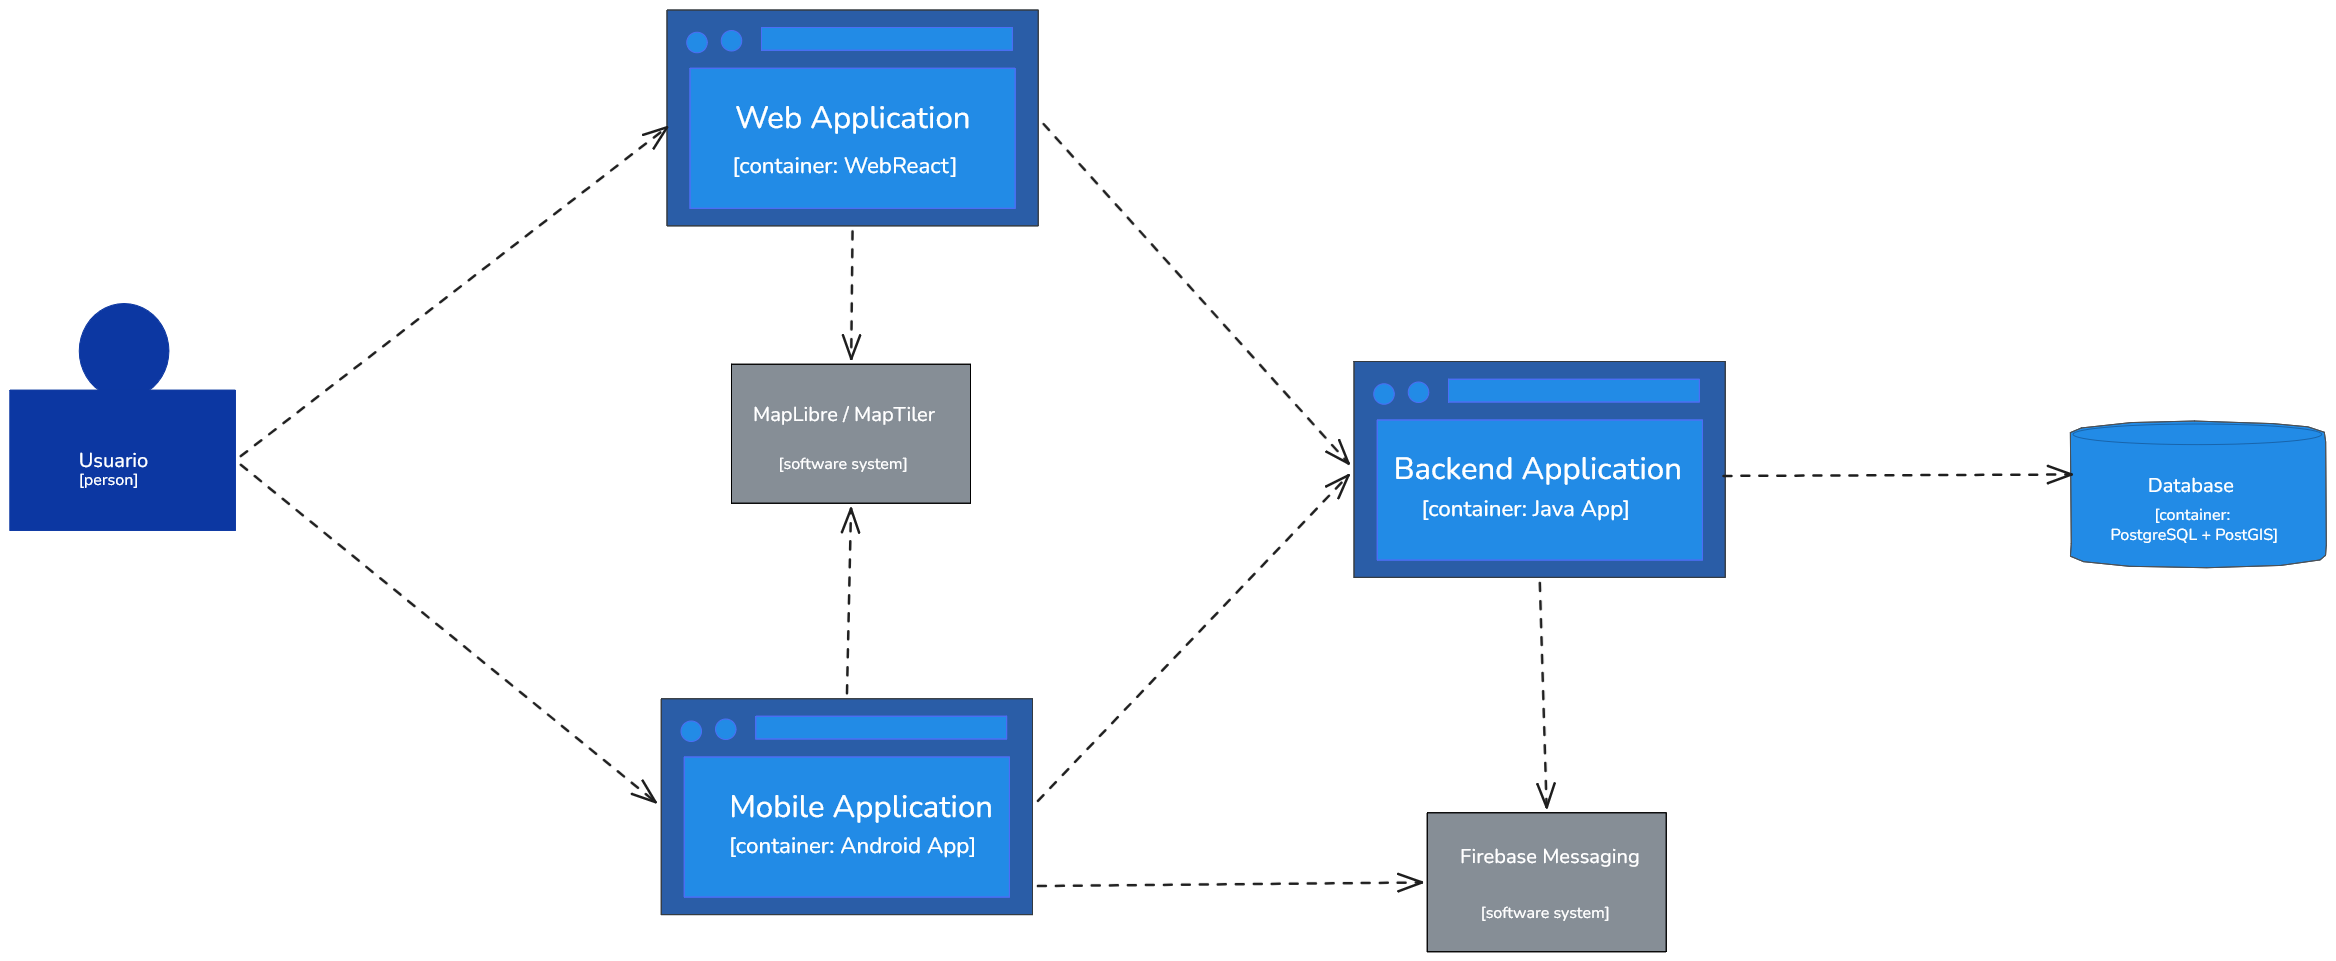
\includegraphics[width=\textwidth]{imaxes/c4/c4_contextual.png}
  \caption{Diagrama C4 de contexto de la aplicación}
  \label{fig:c4-contextual}
\end{figure}

En la figura \ref{fig:c4-contextual} se muestra la relación general entre los usuarios y los distintos sistemas con los que interactúa la aplicación. En esta vista de contexto se aprecia que el sistema central es el backend, que expone una \acrshort{api} \acrshort{rest} consumida tanto por el frontend web como por la aplicación Android. Además, el backend se integra con servicios externos como \acrshort{fcm} para notificaciones push y con una base de datos PostGIS para persistencia geoespacial. Los usuarios interactúan principalmente con el frontend web para gestión y consulta, mientras que la aplicación Android ofrece acceso móvil a información operativa y acciones frecuentes.

%%%%%%%%%%%%%%%%%%%%%%%%%%%%%%%%%%%%%%%%
% Subsistema Backend %
%%%%%%%%%%%%%%%%%%%%%%%%%%%%%%%%%%%%%%%%
\newpage
\section{Subsistema Backend}

\subsection{Objetivos}

El backend tiene como objetivo coordinar el estado de las emergencias, recursos, asignaciones y avisos. Debe exponer una \acrshort{api} \acrshort{rest} que permita al frontend web y a la aplicación Android consultar información operativa, gestionar emergencias, crear asignaciones, enviar avisos y configurar reglas de recomendación. Además, el backend debe garantizar la seguridad mediante autenticación y autorización, así como registrar históricos de las operaciones relevantes para trazabilidad y auditoría.

\subsection{Arquitectura}

La estructura del backend sigue un esquema clásico de Spring Boot. En la capa de entrada se encuentran los controladores \textit{REST}, que reciben las peticiones HTTP y devuelven \textit{DTOs}, que se transforman a representación JSON para ser devueltos. En la capa intermedia se sitúan las fachadas y servicios, donde se implementa la lógica de negocio. En la capa inferior están las entidades JPA y los repositorios, responsables de la persistencia.

\begin{figure}[H]
  \centering
  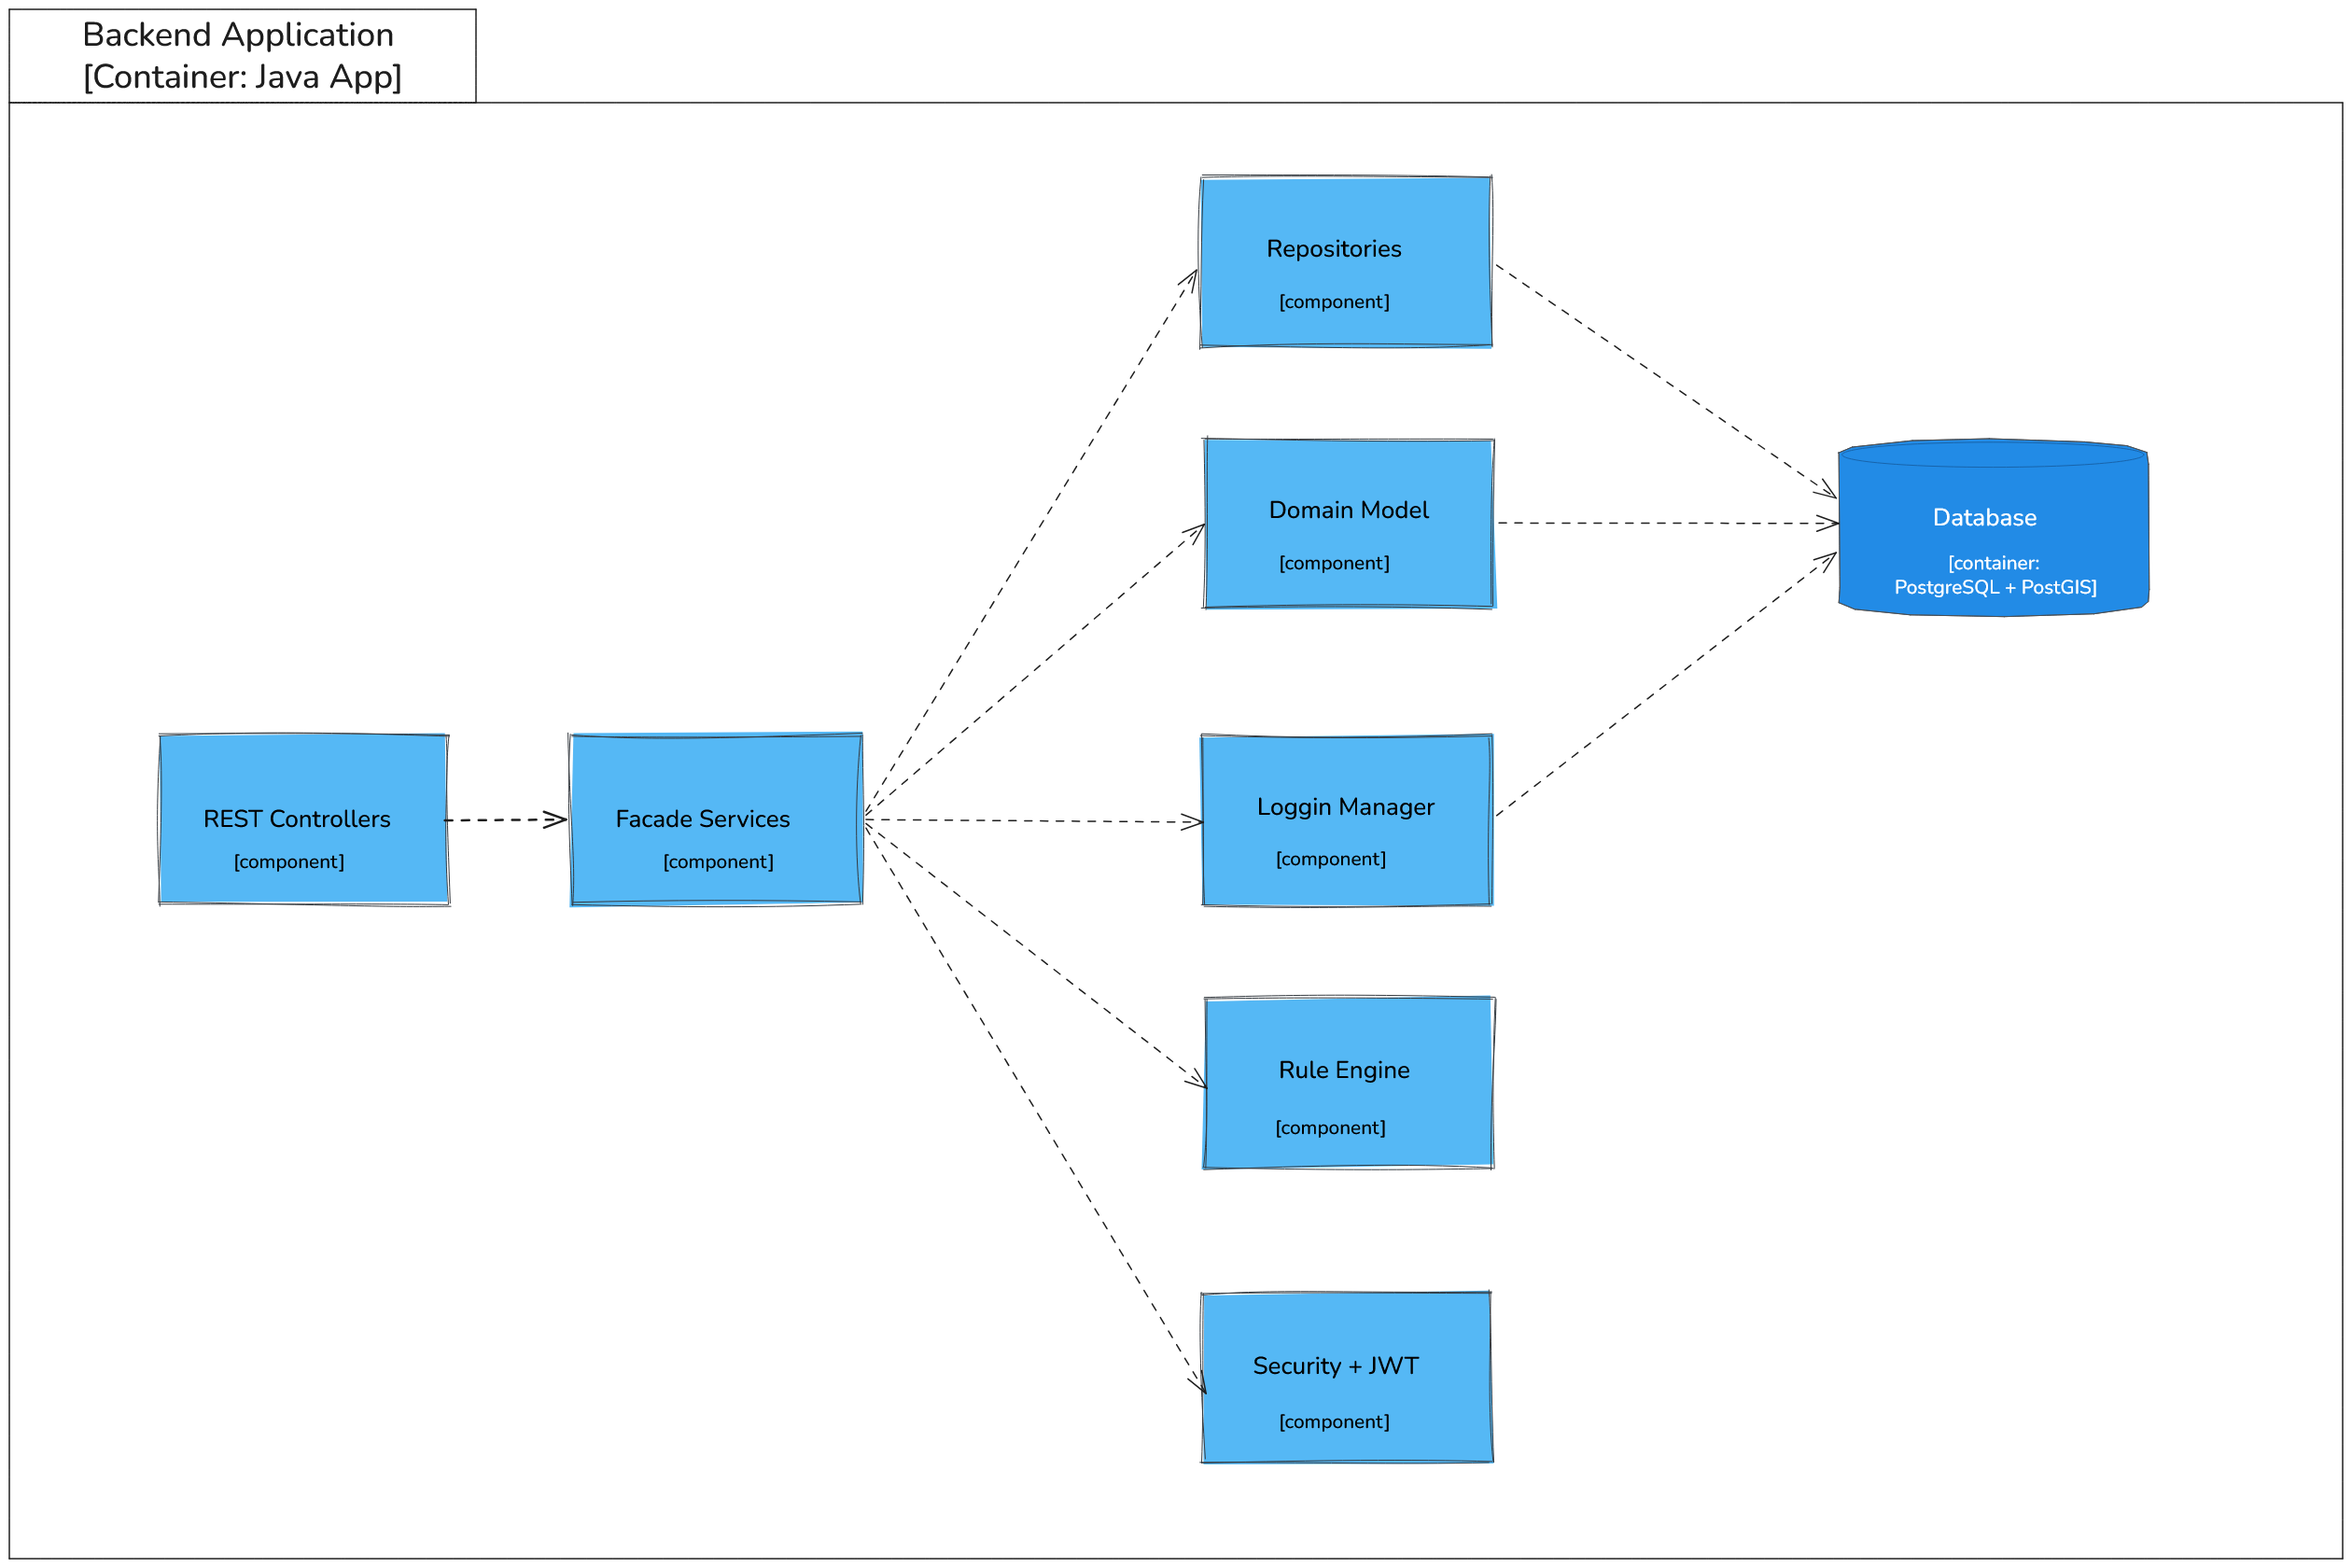
\includegraphics[width=0.7\textwidth]{imaxes/c4/c4_container_backend.png}
  \caption{Diagrama C4 de contenedores del backend}
  \label{fig:c4-container-backend}
\end{figure}

En la figura \ref{fig:c4-container-backend} se aprecia el contenedor backend y su descomposición en controladores, servicios fachada, modelo de dominio, repositorios, seguridad y gestión de históricos. La vista resume la estructura interna sin entrar en componentes más finos. 

Se ha utilizado el color verde para los nuevos componentes añadidos respecto al trabajo previo: la gestión de registros y el motor de reglas de recomendación. Los componentes existentes se han ampliado para dar soporte a las nuevas funcionalidades, como la gestión de asignaciones y la vinculación de emergencias a cuadrantes. Por ejemplo, el componente de dominio se ha extendido con nuevas entidades y relaciones, mientras que las fachadas han incorporado operaciones para gestionar asignaciones y reglas de recomendación.


\subsection{Modelo del dominio}

\subsubsection{Diagrama de entidades}

El modelo de dominio se ha ampliado respecto al trabajo previo. En verde se resaltan las nuevas entidades. El diagrama \ref{fig:modelo-dominio} muestra la evolución: de un dominio centrado en incendios, recursos y avisos a otro que incorpora emergencias, asignaciones, reglas de recomendación y una gestión de históricos más detallada.

\begin{figure}[H]
  \centering
  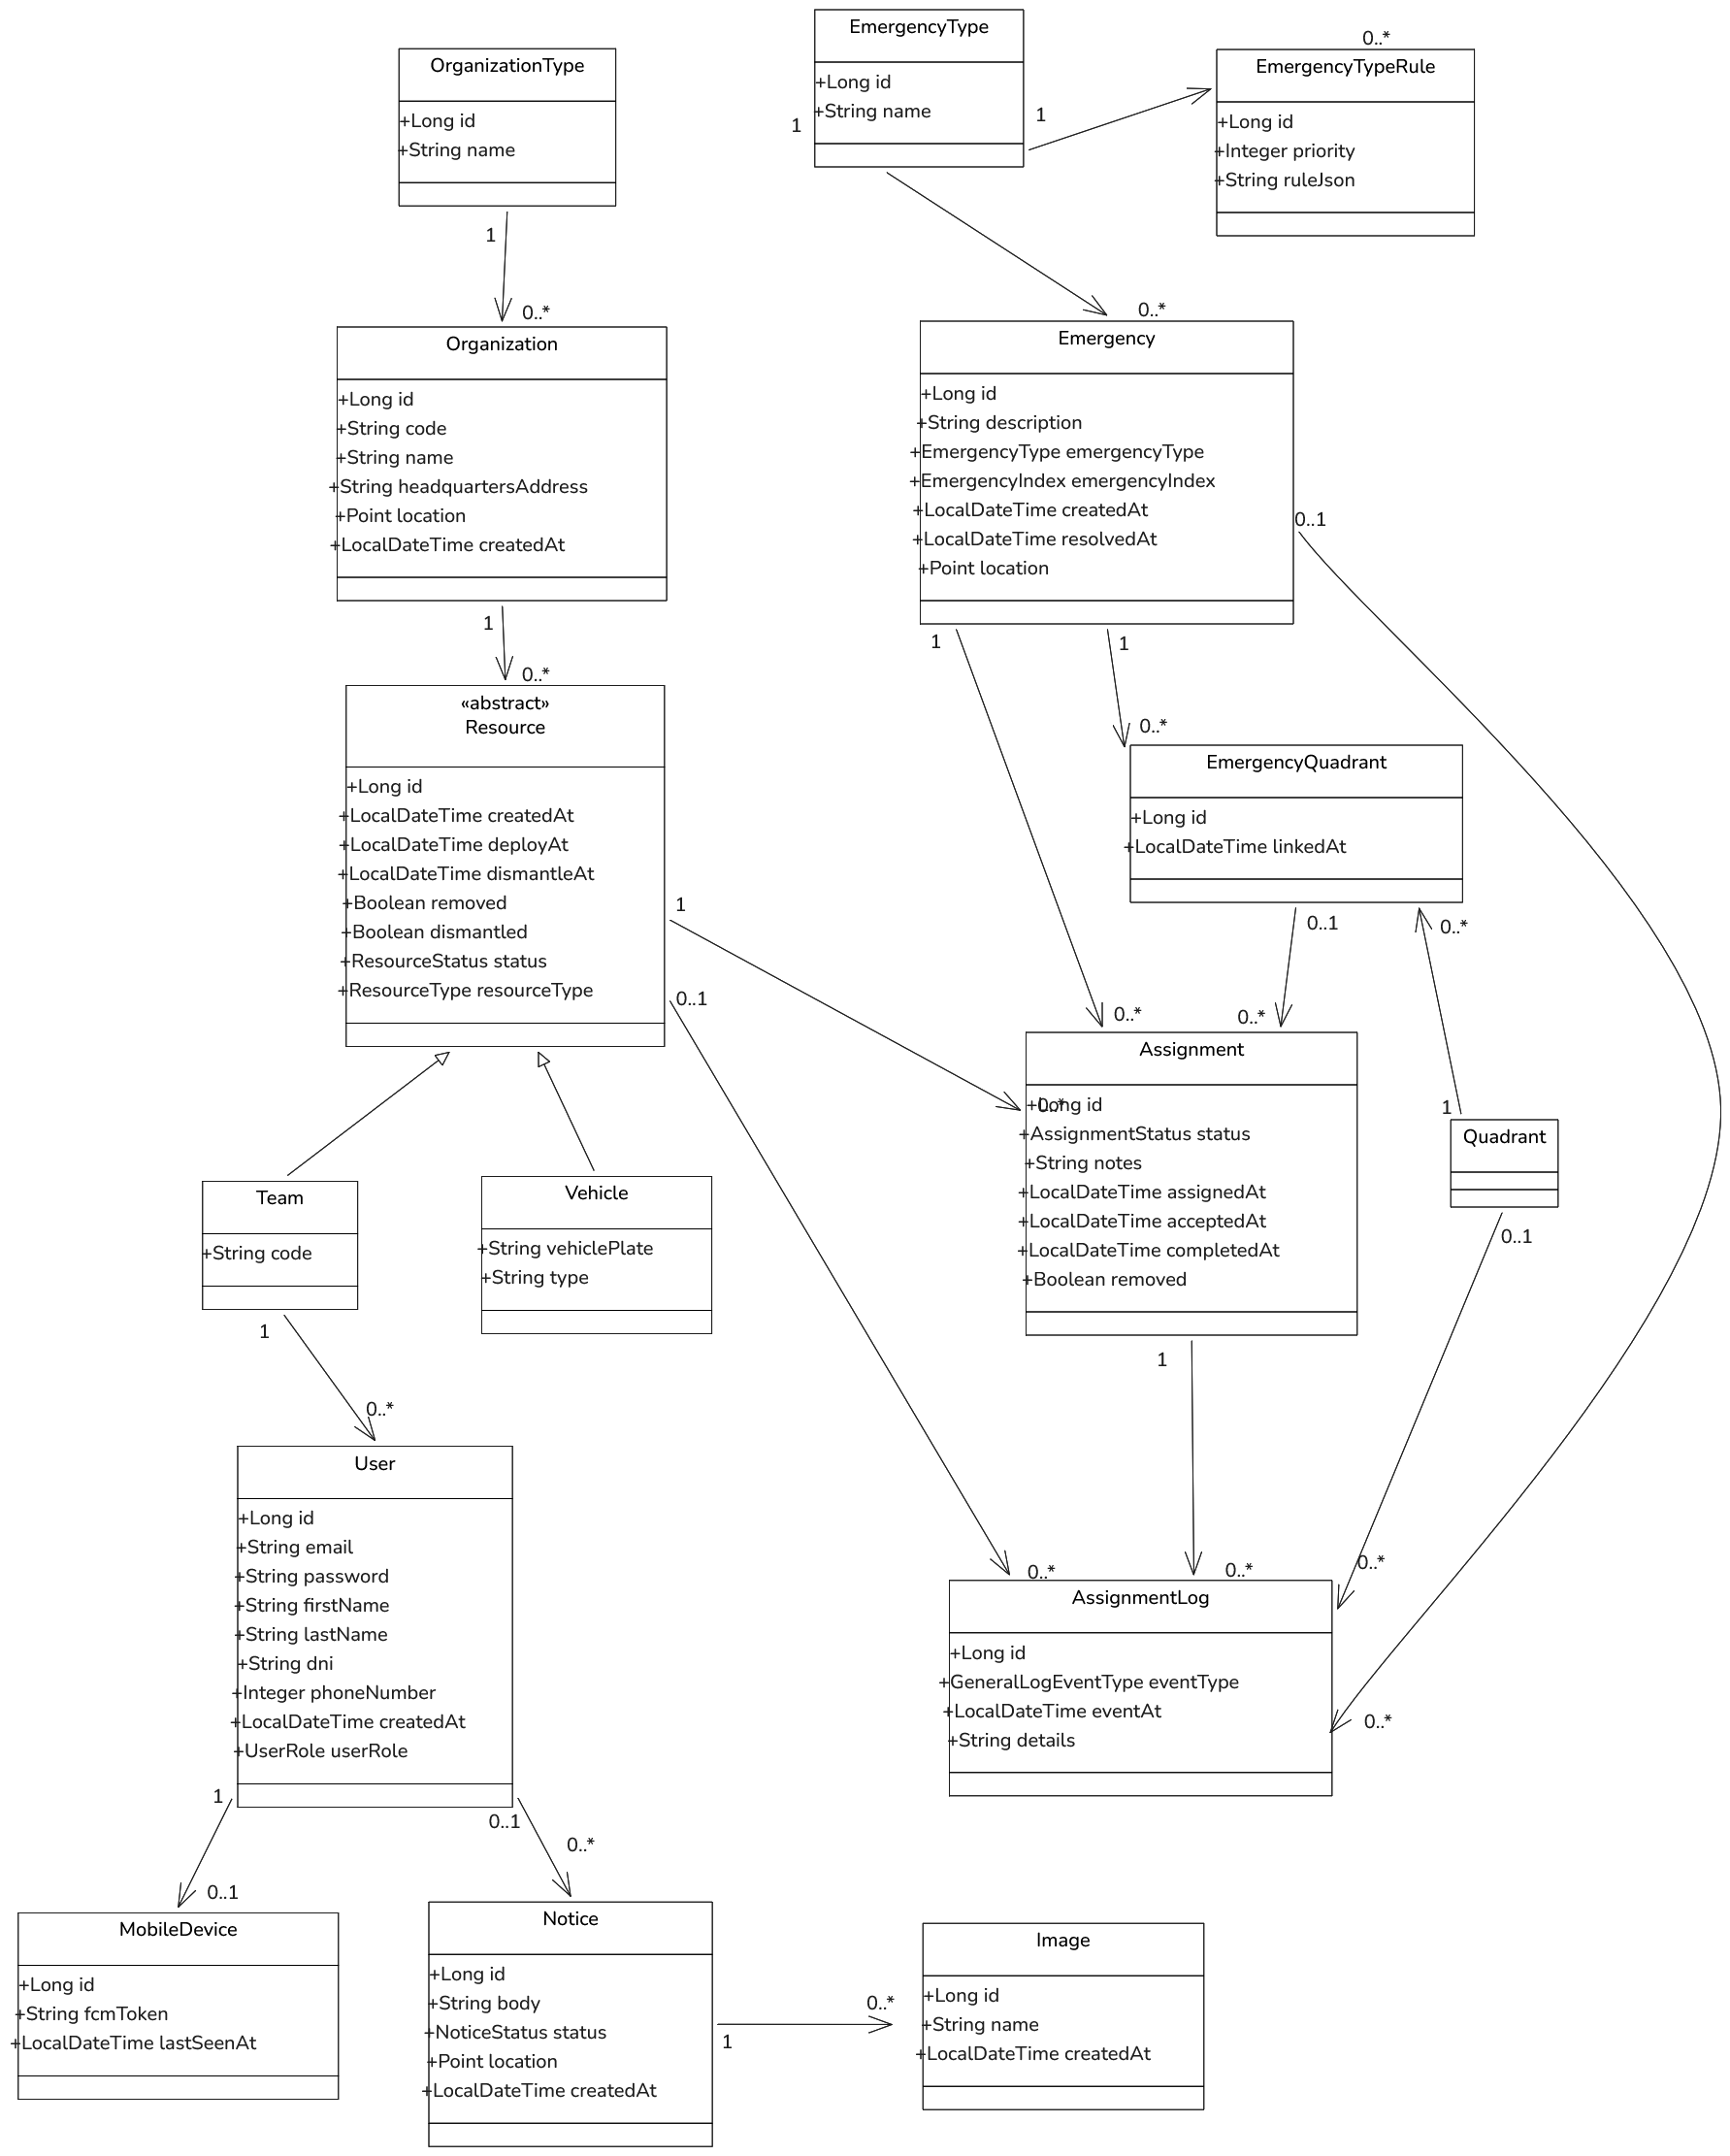
\includegraphics[width=0.9\textwidth]{imaxes/modelo_dominio.png}
  \caption{Diagrama de entidades del modelo de dominio}
  \label{fig:modelo-dominio}
\end{figure}

Frente al trabajo previo, la entidad \textit{Fire} ha sido sustituida por \textit{Emergency}, que amplía el concepto de incidencia y mantiene atributos como descripción, tipo, índice, fechas de creación y resolución, además de admitir tanto localización por punto como vinculación a cuadrantes. Esta ampliación refleja mejor el funcionamiento real de la aplicación, ya que ahora una emergencia puede gestionarse por cuadrantes o por coordenadas.

Otra diferencia relevante es la aparición de \textit{EmergencyQuadrant}, que conserva la relación histórica entre emergencias y cuadrantes con su fecha de vinculación. En la etapa anterior esta información ya existía vinculada al incendio, pero aquí se ha decidido darle una entidad propia para reflejar mejor la evolución de las emergencias a lo largo del tiempo y su relación con los cuadrantes. 

Las asignaciones pasan a tener una entidad propia, \textit{Assignment}, con mayor alcance que en el proyecto anterior. Ahora no solo enlazan recursos con una emergencia, sino que también pueden referirse a un cuadrante concreto o a una emergencia basada en punto, almacenando además su estado, observaciones y marcas temporales del ciclo de vida. Esta ampliación es clave para reflejar los recursos utilizados en las resoluciones de las emergencias.

Los recursos siguen compartiendo la clase base \textit{Resource}, pero su alcance funcional se ha ampliado. \textit{Team} y \textit{Vehicle} heredan de ella y, además de sus datos específicos, ahora participan de forma explícita en el ciclo de despliegue y retirada a través de estados, fechas de despliegue y desmantelamiento y asociaciones con asignaciones. Esto refuerza el papel operativo de ambos tipos de recurso dentro de la aplicación.

En la parte de personal, \textit{User}, \textit{Organization} y \textit{OrganizationType} mantienen la estructura general de la etapa previa, pero su uso se ha ampliado con nuevas relaciones operativas, como la pertenencia a equipos y el registro de dispositivos móviles mediante \textit{MobileDevice}. También se refuerza el papel de \textit{Organization} como contenedor de recursos y unidad de gestión. El bloque de avisos conserva la idea del trabajo anterior con \textit{Notice} e \textit{Image}.

Finalmente, la parte de históricos ya no se apoya únicamente en registros específicos por tipo de recurso, sino en \textit{AssignmentLog}, que unifica la trazabilidad de eventos relacionados con emergencias, cuadrantes y recursos. Esta evolución simplifica la consulta del pasado operativo del sistema y aporta una visión más homogénea de los cambios producidos en la gestión diaria.


\newpage
\subsubsection{Modelo de datos}

El modelo de datos también se ha ampliado de forma notable respecto al trabajo previo. La figura \ref{fig:diagram-bd} resume el esquema relacional actual y permite ver cómo la base de datos ha pasado de una estructura centrada en incendios, recursos y registros históricos separados por tipo a un modelo más homogéneo, orientado a emergencias, asignaciones y trazabilidad operativa.

\begin{figure}[H]
  \centering
  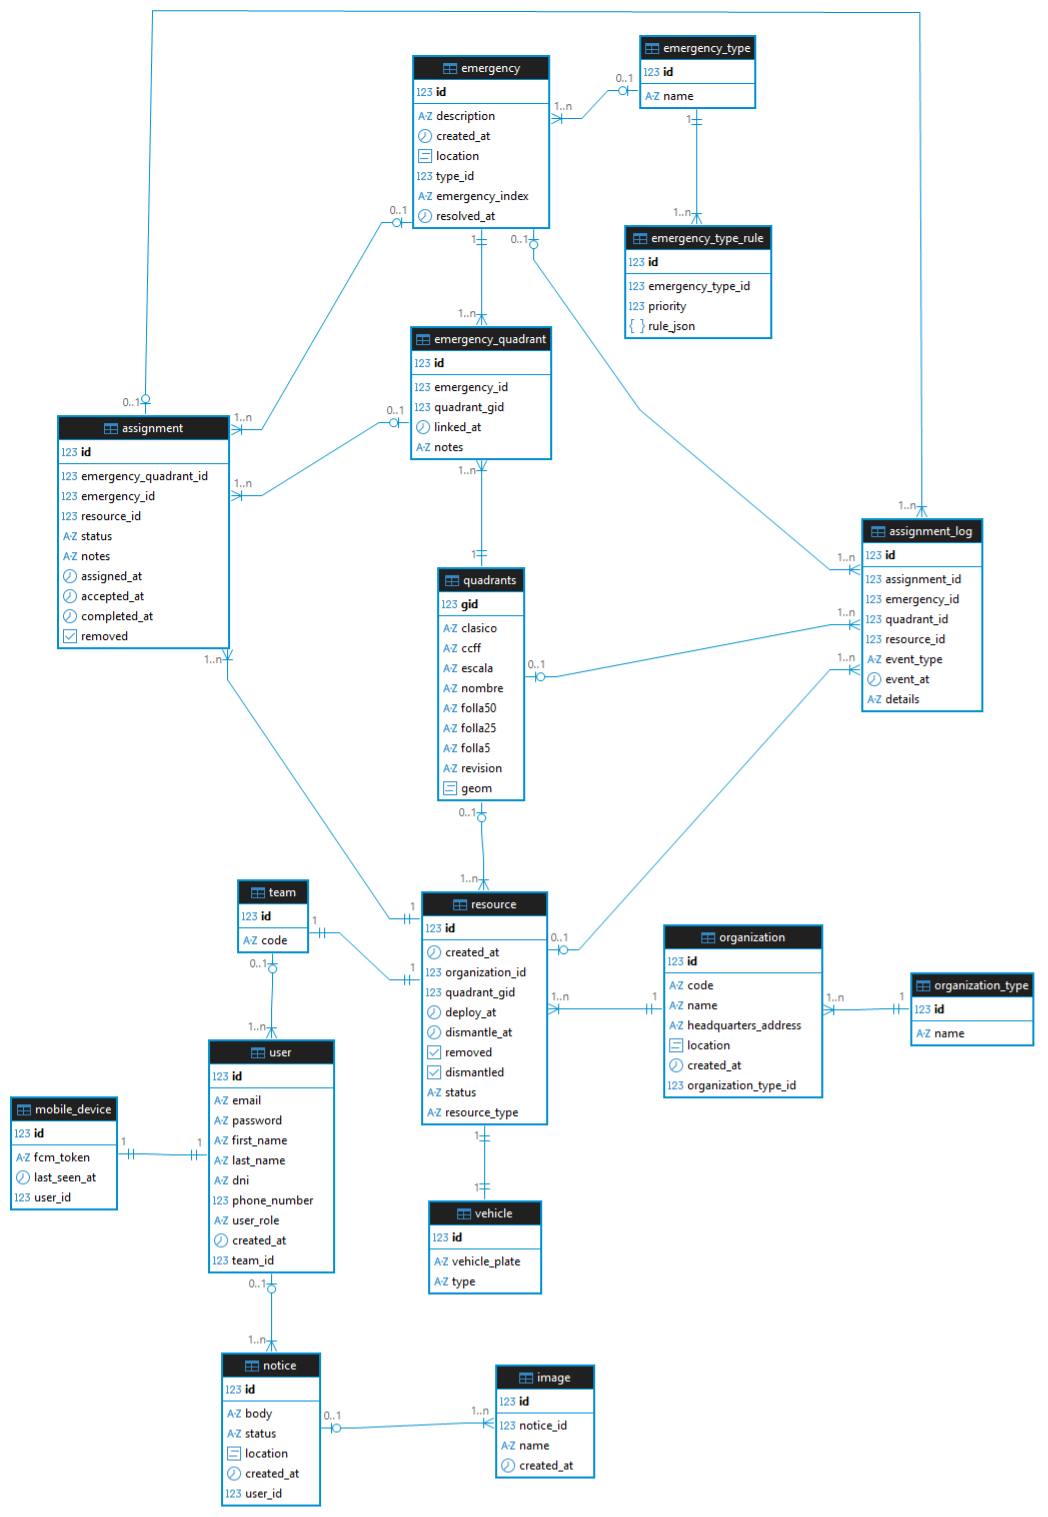
\includegraphics[width=0.82\textwidth]{imaxes/diagram-bd.png}
  \caption{Diagrama relacional de la base de datos}
  \label{fig:diagram-bd}
\end{figure}

En la figura \ref{fig:diagram-bd} se observa que el modelo relacional sigue reproduciendo de forma directa el modelo de dominio, pero con relaciones y tablas adicionales que amplían el alcance funcional del sistema. Frente a la etapa anterior, la aparición de la tabla de \textit{assignment} introduce una entidad central para vincular recursos con emergencias y cuadrantes, mientras que \textit{emergency\_quadrant} consolida la relación entre emergencias y cuadrantes como una relación con histórico propio. Además, se incorpora \textit{emergency\_type\_rule} para almacenar las reglas que alimentan el motor de recomendación, y \textit{mobile\_device} para asociar usuarios con el token FCM utilizado en notificaciones móviles.

También se mantienen las tablas de organizaciones, usuarios, recursos, avisos e imágenes, pero su uso queda ahora integrado en un dominio más amplio. En particular, el antiguo bloque de históricos por recurso se reorganiza alrededor de \textit{assignment\_log}, lo que unifica el registro de eventos y facilita la consulta del pasado operativo. Por último, el modelo conserva campos geoespaciales para almacenar puntos, polígonos y multipolígonos, ya que el sistema sigue trabajando con cuadrantes, localizaciones de emergencias y localizaciones de organizaciones.

\subsubsection{Consideraciones adicionales de modelado de datos}

La mayoría de entidades siguen utilizando claves primarias autogeneradas, lo que simplifica la persistencia y evita lógica manual de asignación de identificadores. Las relaciones entre entidades se definen con anotaciones JPA, principalmente \textit{@ManyToOne}, \textit{@OneToMany} y \textit{@OneToOne}, según la cardinalidad real del dominio.

Se mantiene la política de carga perezosa en las relaciones que pueden crecer en tamaño, como usuarios de un equipo o cuadrantes de una emergencia, pero ahora esa decisión cobra más importancia porque el número de asociaciones ha aumentado. En particular, las relaciones de asignaciones, logs y reglas de recomendación añaden nuevas rutas de navegación entre entidades que conviene cargar solo cuando resultan necesarias.

También se han reforzado las validaciones de Bean Validation, se han añadido restricciones de unicidad y se han definido enumeraciones para campos con valores limitados, como el estado de asignaciones o el tipo de emergencia. Esto afecta tanto a entidades ya existentes, como \textit{Resource} o \textit{User}, como a las nuevas entidades relacionadas con asignaciones y recomendaciones. En \textit{Resource} se centralizan pequeñas reglas de coherencia, por ejemplo el borrado de \textit{deployAt} cuando el recurso vuelve al estado disponible, lo que reduce la dispersión de lógica repetida.

Otro cambio relevante es que en el trabajo anterior la parte de históricos se organizaba por tipo de recurso, con entidades específicas para cada uno. Actualmente se ha optado por un modelo más unificado con \textit{AssignmentLog}, que registra eventos relacionados con asignaciones, emergencias y cuadrantes sin necesidad de separar por tipo de recurso.

\subsection{Capa de acceso a datos}

La capa de acceso a datos se implementa mediante repositorios que extienden \textit{JpaRepository}. Esto proporciona operaciones CRUD sin necesidad de escribir consultas para los casos más comunes. Cuando hace falta un acceso más específico, se añaden métodos derivados por nombre o consultas personalizadas.

El diagrama de la figura \ref{fig:diagram-repository} recoge todos los repositorios del sistema con sus métodos más relevantes. Entre ellos destacan aquellos que incorporan la lógica de acceso más compleja: \textit{AssignmentRepository} combina múltiples criterios de filtrado (cuadrante, emergencia y recurso) en un solo método \texttt{findByFilters}, mientras que \textit{QuadrantRepository} incluye una consulta geoespacial nativa para el cálculo de superficies en hectáreas y una consulta que determina qué cuadrantes tienen emergencias activas. \textit{UserRepository} expone métodos que localizan usuarios por su equipo y rol, necesarios para dirigir las notificaciones push a los miembros del equipo asignado. Por su parte, \textit{TeamRepository} y \textit{VehicleRepository} proporcionan consultas de proximidad geográfica (\texttt{findAvailableClosestToLocation}) que alimentan el motor de recomendación de recursos. El resto de repositorios siguen una estructura más simple, limitándose en su mayoría a las operaciones CRUD heredadas.

\begin{figure}[H]
  \centering
  \includegraphics[width=\textwidth]{imaxes/diagrama-repository.png}
  \caption{Diagrama de repositorios}
  \label{fig:diagram-repository}
\end{figure}


\subsection{Capa de lógica de negocio}

La lógica de negocio se organiza en \textit{facades} e interfaces de servicio, tal como se representa en la figura \ref{fig:diagram-negocio}. \textit{PersonalManagementFacade} agrupa operaciones de organizaciones y usuarios, \textit{ResourceManagementFacade} agrupa equipos y vehículos, \textit{EmergencyManagementService} centraliza las operaciones sobre emergencias y cuadrantes, \textit{AssignmentService} gestiona el ciclo de vida de las asignaciones y \textit{LogManagementService} se encarga de registrar eventos históricos.

En la fachada de personal se gestionan las operaciones de registro, inicio de sesión, edición de perfil, cambio de contraseña, asociación de dispositivos móviles y modificación de roles. En la fachada de recursos, se permiten altas, modificaciones, bajas lógicas y gestión de miembros en equipos. Las organizaciones también se crean y se actualizan desde esta capa.

La parte de emergencias concentra las operaciones de creación, actualización, resolución y vinculación a cuadrantes o puntos. La lógica verifica restricciones de negocio como no modificar una emergencia resuelta o no vincular una emergencia a un punto si ya está asociada a cuadrantes. Como refleja la figura \ref{fig:diagram-negocio}, \textit{EmergencyManagementService} es el servicio con mayor número de operaciones, lo que subraya su papel central en la gestión del sistema.

Junto a estos servicios generales, el diagrama recoge los dos ámbitos más relevantes de la nueva funcionalidad. Por un lado, \textit{AssignmentService} gestiona el ciclo de vida completo de las asignaciones (creación, transiciones de estado y eliminación lógica), apoyándose en \textit{LogManagementService} para registrar cada evento y en \textit{AssignmentNotificationService} para notificar a los miembros del equipo asignado. Por otro lado, los servicios de recomendación (\textit{EmergencyRecommendationService}, \textit{RecommendationRuleManagementService}) implementan el motor de reglas que sugiere recursos de forma semiautomática según el tipo de emergencia y la proximidad geográfica. Estas colaboraciones entre servicios, visibles en la figura, constituyen el núcleo de la nueva lógica de negocio introducida en el proyecto.

\begin{figure}[H]
  \centering
  
\includegraphics[width=\textwidth]{imaxes/diagrama-negocio.png}
  \caption{Diagrama de servicios de lógica de negocio}
  \label{fig:diagram-negocio}
\end{figure}


Las asignaciones son el núcleo más dinámico del sistema. En el siguiente diagrama de secuencia \ref{fig:diagram-assignment} se muestra el flujo de creación de una asignación. El usuario selecciona la emergencia, el cuadrante y el recurso, y envía la petición al backend. \textit{AssignmentService} valida los datos, comprueba que el recurso esté disponible y que la emergencia y el cuadrante existan. Si todo es correcto, se crea la asignación, se registra en el histórico y se envía una notificación al dispositivo móvil del usuario asignado.

\begin{figure}[H]
  \centering
  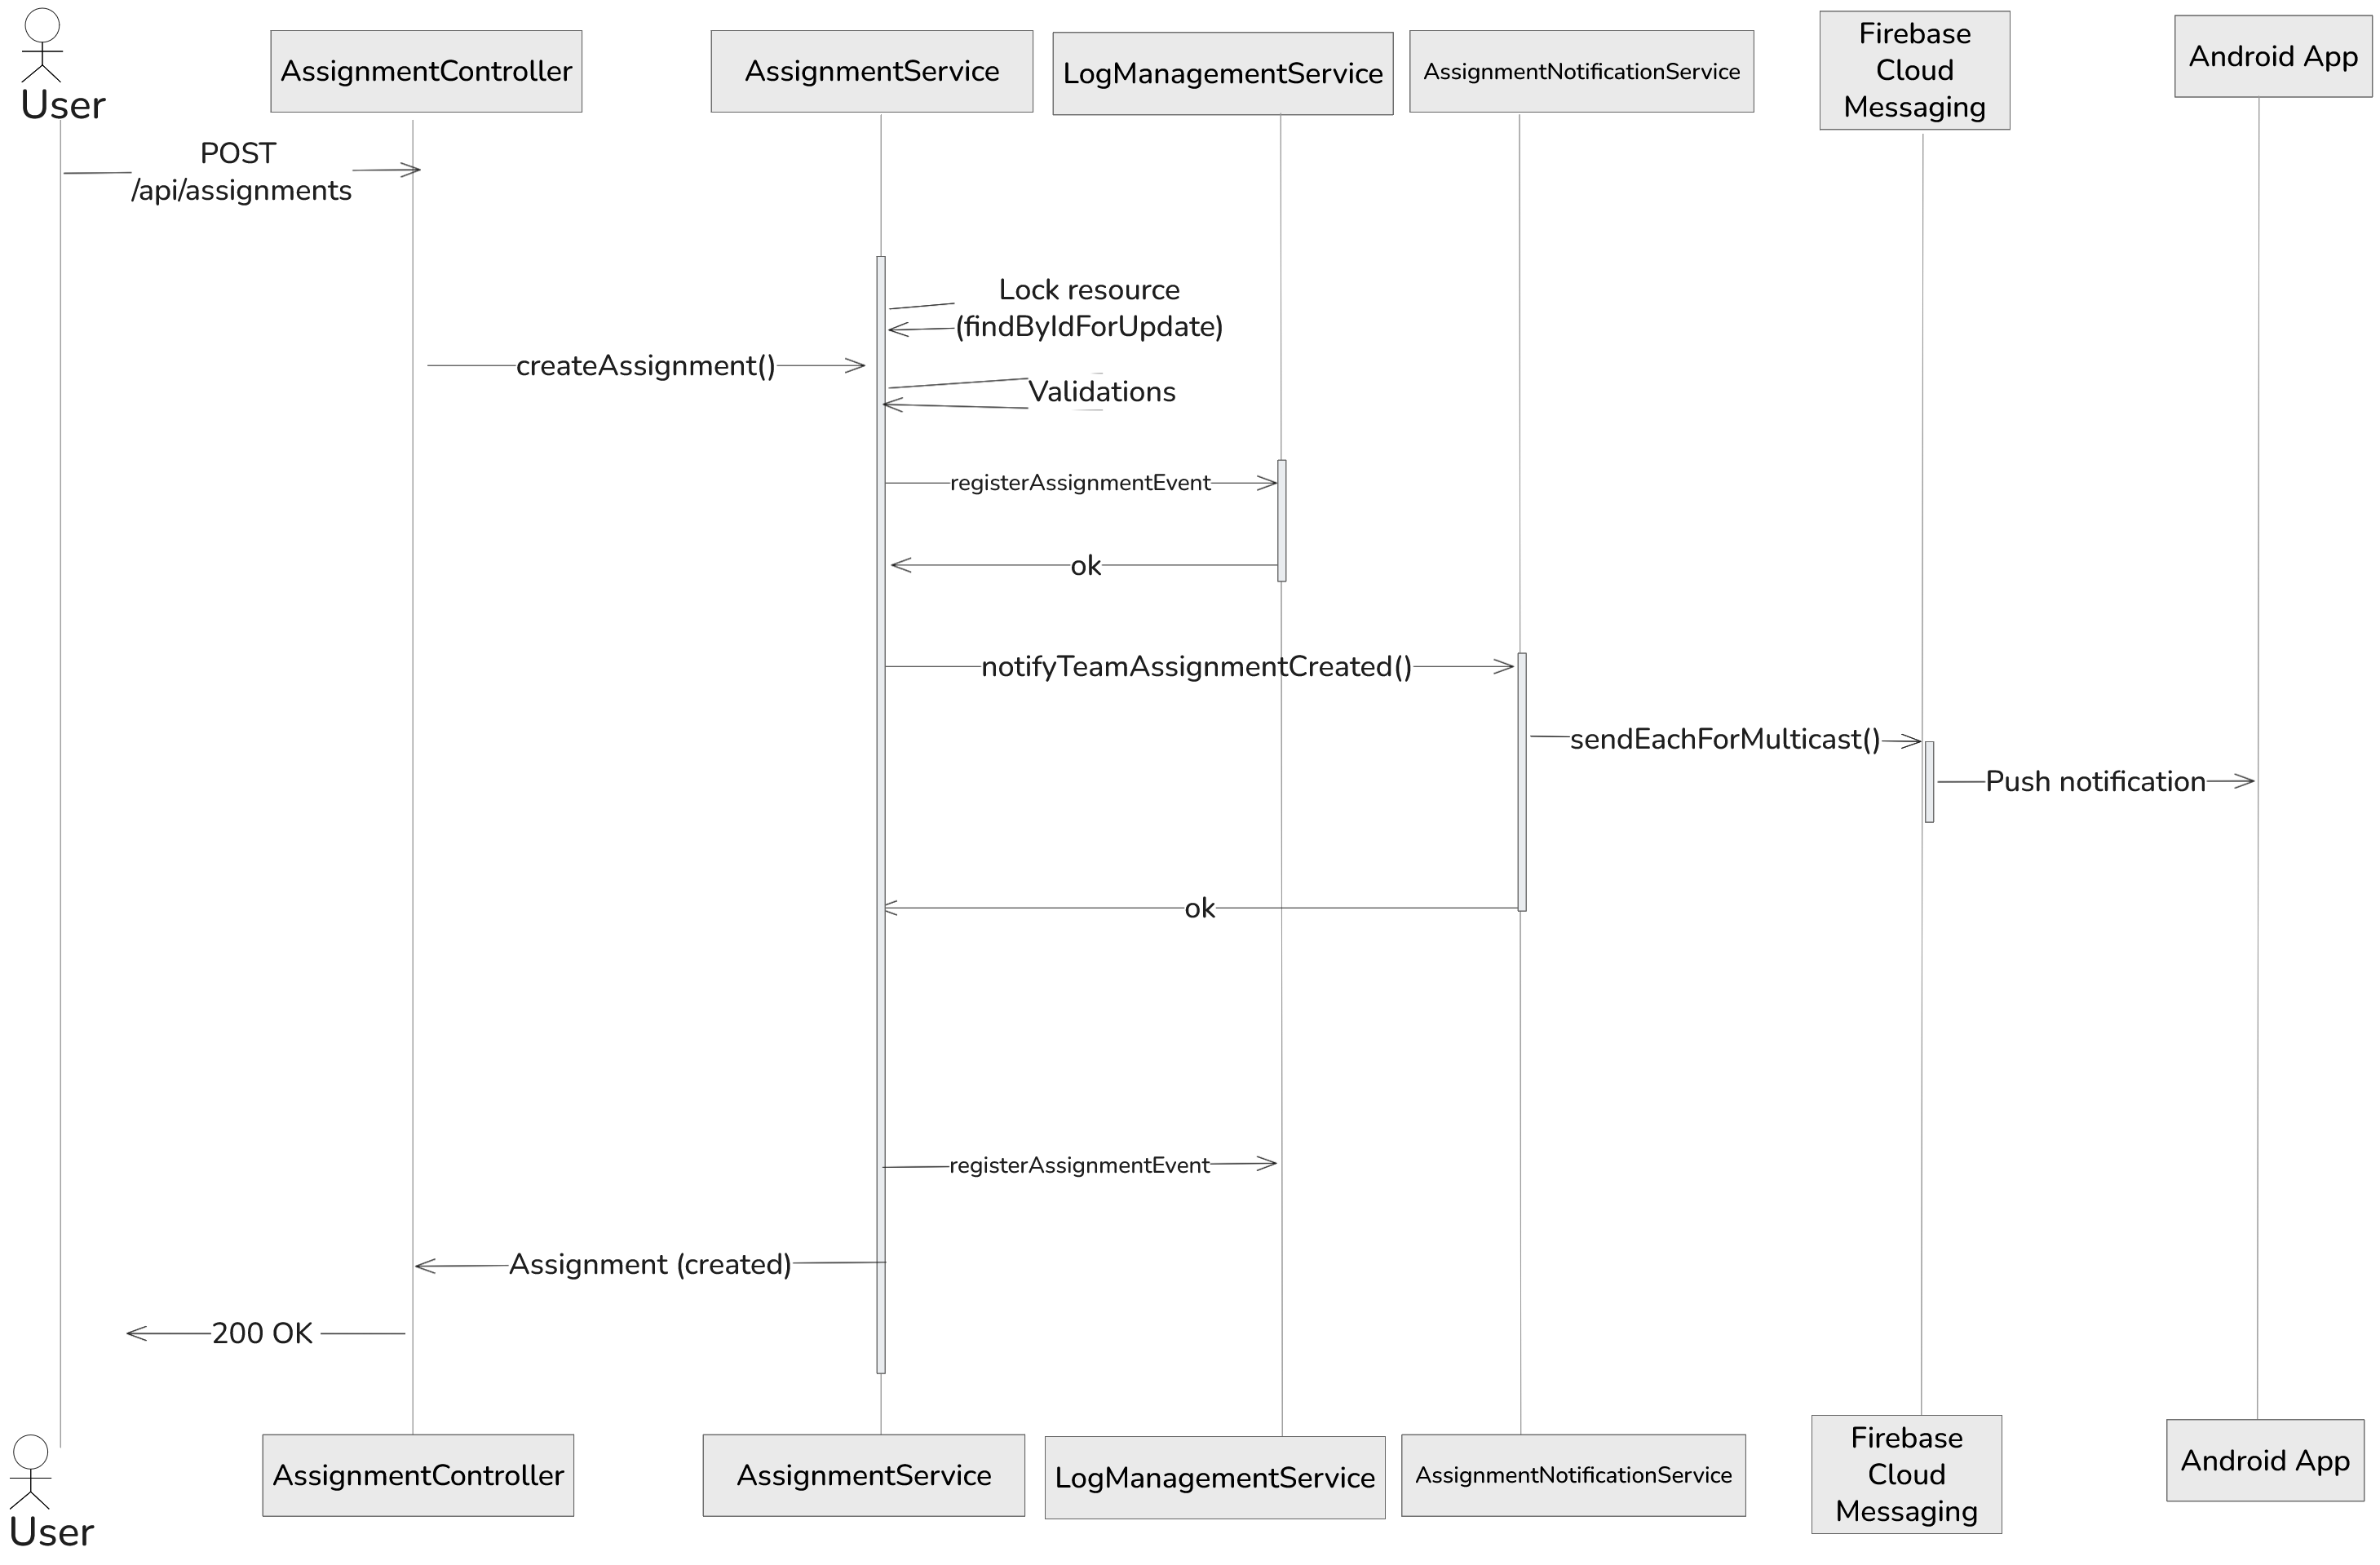
\includegraphics[width=\textwidth]{imaxes/diagrama-secuencia-asignación.png}
  \caption{Diagrama de secuencia de asignación de recursos a una emergencia}
  \label{fig:diagram-assignment}
\end{figure}

Cuando una asignación cambia de estado, el servicio actualiza el recurso asociado, marca la fecha de despliegue o retirada y vuelve a registrar el evento correspondiente. En caso de resolución de la emergencia, las asignaciones pendientes se eliminan lógicamente y las aceptadas se completan automáticamente.

La recomendación semiautomática de recursos se apoya en la entidad \textit{EmergencyTypeRule}, que asocia un tipo de emergencia con una regla en formato JSON estructurado en dos partes: una condición \textit{when} que define el perfil de emergencia (p. ej., tipo concreto, umbral de índice) y una acción \textit{then} que especifica la propuesta (número de equipos, número de vehículos, distancia máxima en kilómetros y tipo de organización preferente). El servicio de edición valida la corrección sintáctica del JSON antes de persistirlo. En tiempo de ejecución, \textit{EmergencyRecommendationService} recupera las reglas ordenadas por prioridad y las evalúa secuencialmente mediante el patrón Chain of Responsibility (descrito en la sección \ref{sec:patrones}); la primera regla cuya condición se cumple determina los parámetros de la recomendación. A partir de ahí, el motor ejecuta consultas de proximidad geográfica (\texttt{findAvailableClosestToLocation}) contra los repositorios de equipos y vehículos para localizar los recursos disponibles más cercanos al punto de la emergencia, aplicando los filtros de distancia máxima y tipo de organización indicados por la regla.

\subsection{Capa de servicios web}

\subsubsection{Diseño de controladores}

Una de las diferencias más importantes es que los controladores se generan a partir de la especificación \textit{OpenAPI}. En la etapa anterior la definición de endpoints dependía de clases controladoras creadas manualmente, mientras que aquí se parte de la descripción de la API y el código generado proporciona la base de las interfaces de controladores y de los contratos de entrada y salida.

Es importante aclarar que se han migrado los endpoints existentes a esta nueva forma de trabajo, lo que ha supuesto un esfuerzo de adaptación pero ha permitido mantener la coherencia en el resto del proyecto. Esta migración es agnóstica respecto a la estructura interna del backend, ya que el código generado se integra con las fachadas y servicios de lógica de negocio sin necesidad de modificar su organización.

Este enfoque reduce errores de sincronización entre documentación e implementación, y facilita que los cambios en la API se propaguen de forma consistente. Los controladores siguen siendo responsables de exponer la operación HTTP, pero la estructura general, los tipos de petición y respuesta y parte de la firma de los endpoints quedan alineados con el contrato definido en \textit{OpenAPI}.

\begin{figure}[H]
  \centering
  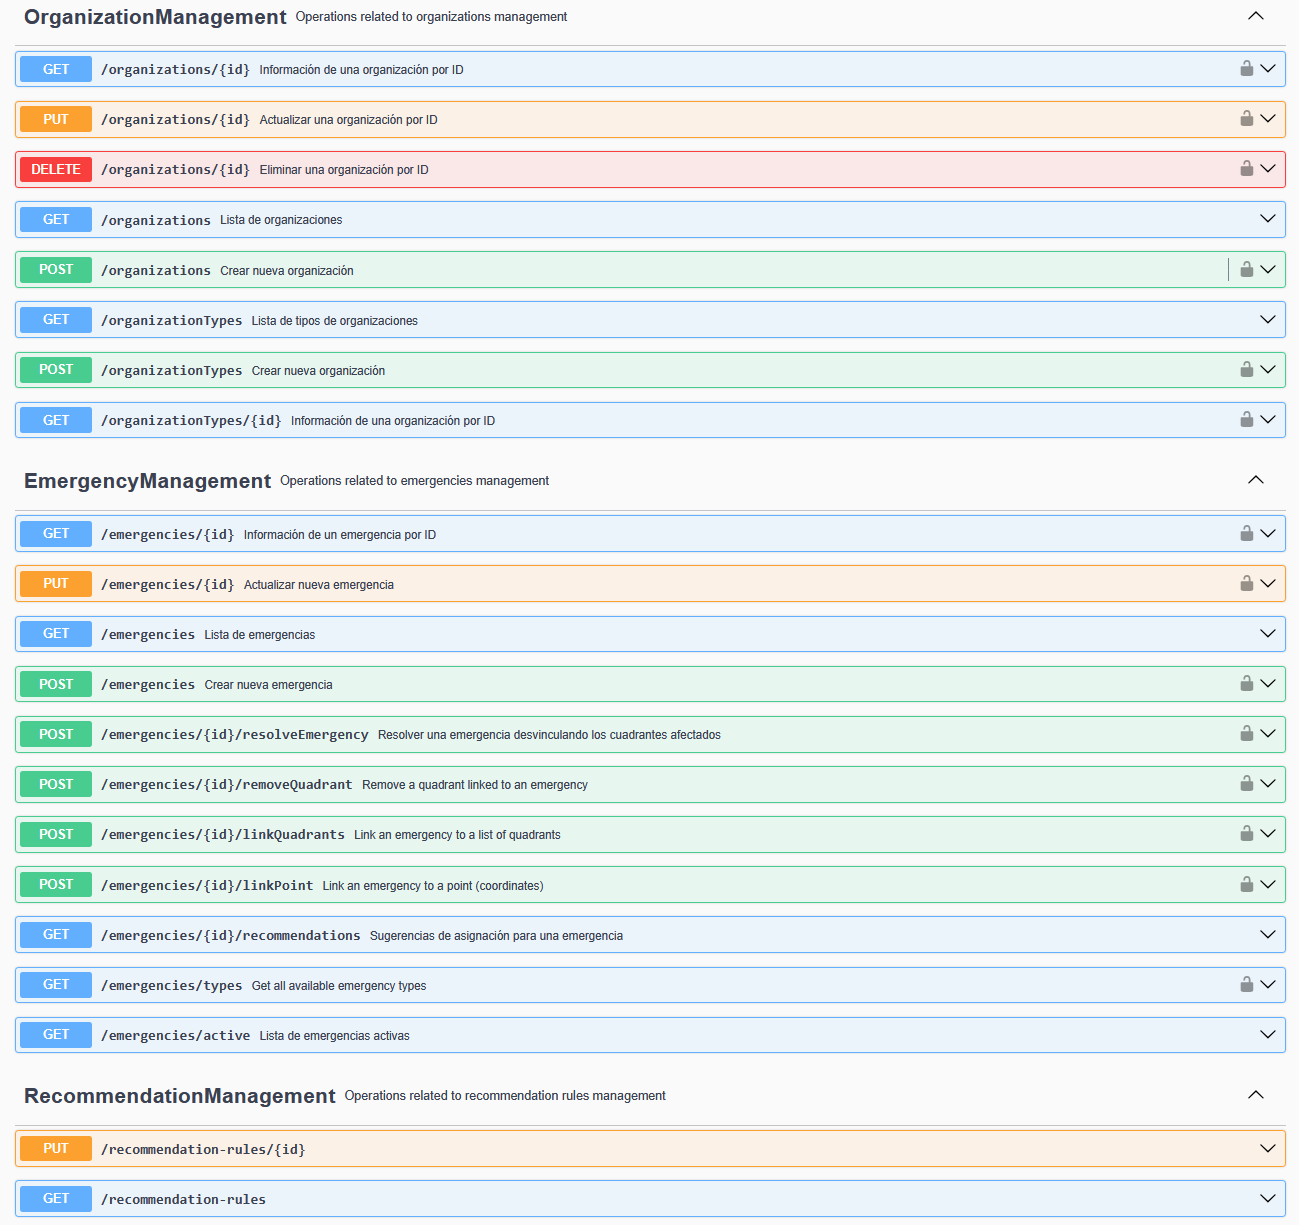
\includegraphics[width=\textwidth]{imaxes/swagger.png}
  \caption{Colección de endpoints documentados en Swagger}
  \label{fig:swagger-collection}
\end{figure}

En la figura \ref{fig:swagger-collection} se muestra la documentación generada mediante Swagger, que refleja los bloques de gestión de organización, de emergencias y de recomendación. El resto de bloques también se ha documentado, pero se han omitido por limitaciones de espacio. En esta vista se observan las ventajas del enfoque \textit{API-first}: la documentación se genera automáticamente a partir del contrato OpenAPI, lo que ayuda a mantenerla sincronizada con la implementación real de los endpoints. Además, permite comprobar de forma centralizada los recursos disponibles, los métodos HTTP asociados y la estructura general de la interfaz pública del backend. También se aprecian los endpoints que requieren autenticación y los accesibles para usuarios anónimos.


\subsubsection{Gestión de errores e internacionalización}

La gestión de errores se centraliza en la clase \textit{GlobalControllerExceptionHandler}. Allí se traducen excepciones de instancia, de dominio y de validación a respuestas HTTP adecuadas y mensajes localizados. Este mecanismo viene del trabajo previo que, con pequeñas adaptaciones, se ha mantenido en la evolución de la aplicación. La internacionalización de mensajes se realiza mediante ficheros de propiedades, y el idioma activo se propaga desde el frontend o la aplicación Android a través de cabeceras HTTP. 

\subsubsection{Control de acceso}

La configuración de seguridad se define en la clase \textit{SecurityConfig}. El backend funciona con sesión sin estado y token JWT. Se autorizan explícitamente los endpoints según el rol: los usuarios anónimos pueden iniciar sesión, registrarse y consultar parte de la información pública; los roles de miembro, gestor y coordinador acceden a recursos y emergencias según sus permisos; y las operaciones de asignación y recomendación quedan restringidas a gestores y coordinadores.

Este bloque también se ha mantenido prácticamente sin cambios estructurales, porque la política de permisos seguía siendo válida para la evolución de la aplicación. La aplicación también registra dispositivos móviles mediante la clase \textit{MobileDevice}, lo que permite enlazar el usuario con su token FCM y habilitar notificaciones push.

\subsection{Librerías y servicios externos}

Además de la persistencia y la seguridad, el backend integra varias librerías y servicios externos. Se usa PostGIS para operaciones geoespaciales, Jackson para el manejo del JSON de reglas de recomendación, y \acrshort{fcm} para notificaciones móviles. También se apoya en una capa de mapeo entre entidades y \textit{DTOs} para desacoplar la API pública del modelo interno.

%%%%%%%%%%%%%%%%%%%%%%%%%%%%%%%%%%%%%%%%
% Subsistema Frontend %
%%%%%%%%%%%%%%%%%%%%%%%%%%%%%%%%%%%%%%%%
\section{Subsistema Frontend}

\begin{figure}[H]
  \centering
  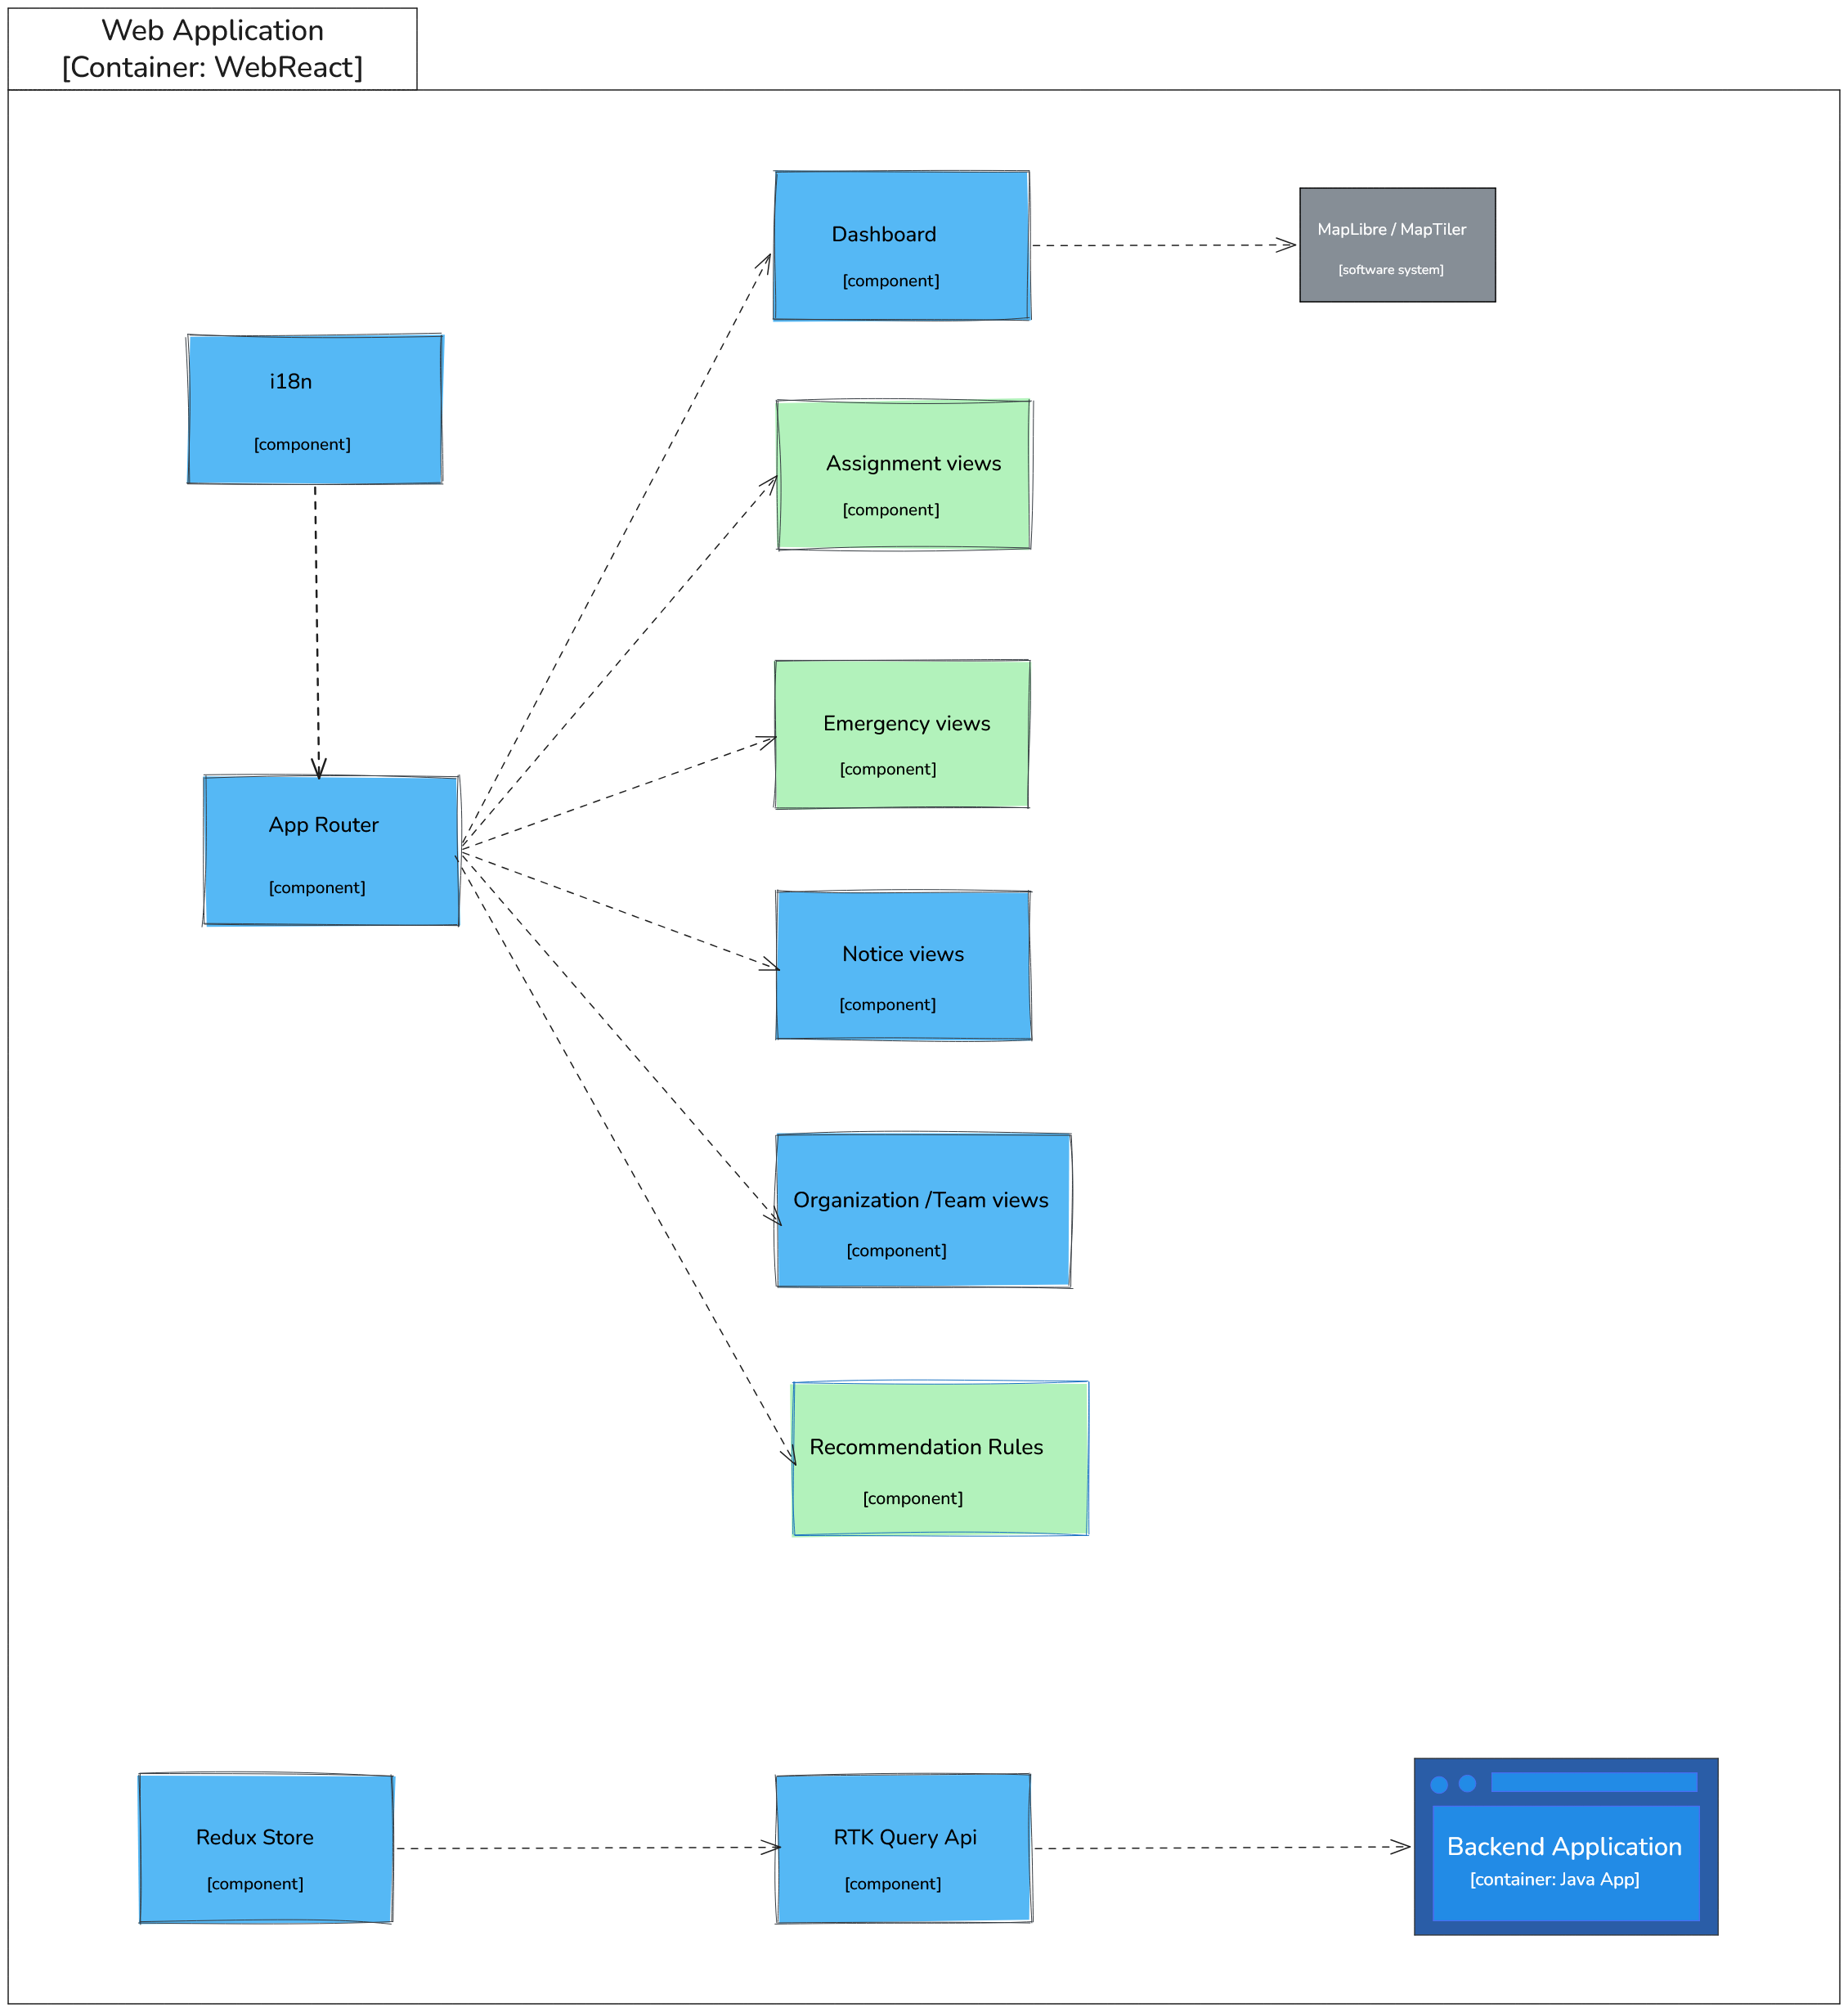
\includegraphics[width=\textwidth]{imaxes/c4/c4_container_frontend.png}
  \caption{Diagrama C4 de contenedores del frontend}
  \label{fig:c4-container-frontend}
\end{figure}

La interfaz se organiza por dominios funcionales reflejados en el diagrama \ref{fig:c4-container-frontend} y se apoya en un store Redux que separa el estado de sesión, el tema visual y los datos de dominio (emergencias, asignaciones, recursos) en slices independientes. Los componentes nuevos o modificados aparecen resaltados en verde.

El mapa (\textit{LandingMap}) representa cada emergencia con un icono y color distintos según su tipología (incendio, inundación, derrumbe, riesgo industrial) y su estado (activa, resuelta). Los cuadrantes se dibujan como polígonos semitransparentes con borde y relleno diferenciados según si están vinculados a una emergencia activa, y los recursos desplegados se muestran como marcadores adicionales sobre el cuadrante correspondiente. Toda la capa cartográfica se apoya en MapLibre con estilos servidos por MapTiler.

La vista de creación de asignaciones presenta tres selectores encadenados: emergencia, cuadrante (solo si la emergencia lo admite) y recurso disponible. Al seleccionar la emergencia, el frontend filtra los cuadrantes vinculados a ella y, al elegir un recurso, valida visualmente que no esté ocupado mostrando su estado en la interfaz antes de enviar la petición. La vista de reglas de recomendación expone un editor JSON con resaltado de sintaxis básico y validación local antes del envío, además de controles para reordenar la prioridad de las reglas mediante arrastre. Los listados de emergencias, asignaciones y avisos incorporan filtros combinados por tipo, estado y fechas, todos gestionados como parámetros de ruta para mantener el estado del filtro entre navegaciones.

%%%%%%%%%%%%%%%%%%%%%%%%%%%%%%%%%%%%%%%%
% Subsistema Android %
%%%%%%%%%%%%%%%%%%%%%%%%%%%%%%%%%%%%%%%%
\section{Subsistema Android}

\subsection{Objetivos}

La aplicación Android complementa al frontend web permitiendo consultar información operativa y ejecutar acciones frecuentes desde el móvil. Debe mostrar mapa, emergencias, organizaciones, perfil, avisos, equipo propio y asignaciones, además de soportar el envío de avisos con imagen y localización.

La interfaz móvil también debe adaptarse al idioma del usuario y mantener coherencia visual con la versión web, aunque con una navegación propia más adecuada al contexto táctil.

Además, la app está pensada como un cliente ligero orientado a la consulta rápida y a la reacción en campo. Por ello concentra en el dispositivo funciones de visualización, notificación y aceptación de asignaciones, mientras delega la lógica de negocio en el backend.

Para mantener la sesión y ciertos parámetros de uso, la aplicación almacena localmente información básica en \textit{SharedPreferences} bajo \textit{app\_prefs}. Ahí se guardan el token JWT, el identificador del usuario, el nombre mostrado, el correo, el teléfono, el DNI, el rol y el idioma activo. Este almacenamiento se usa para restaurar la sesión, aplicar cabeceras de autorización y conservar la configuración lingüística entre ejecuciones.

\subsection{Arquitectura}

La aplicación Android combina una actividad principal con pantallas implementadas en Compose y flujos concretos basados en Activities y Fragments. Desde esa actividad se resuelve la navegación entre pantallas y se mantiene el acceso centralizado al estado de sesión y a las funciones principales.

La aplicación se apoya en una capa de acceso a red centralizada en \textit{HttpClient}, que se encarga de gestionar las peticiones al backend, incluyendo la lectura del token JWT desde preferencias compartidas y la gestión de hosts locales para facilitar el desarrollo. Todas las pantallas reutilizan esa capa para evitar duplicar lógica de conexión, lectura del token y tratamiento del contenido JSON.


La parte de emergencias se apoya en varias pantallas complementarias. \textit{MapScreen} dibuja cuadrantes activos y emergencias sobre MapLibre. \textit{EmergenciesScreen} muestra el listado filtrable de emergencias. \textit{EmergencyDetailScreen} presenta el detalle de una emergencia y, cuando existe localización por punto, consulta el cuadrante correspondiente y recupera las asignaciones vinculadas. \textit{QuadrantResourcesScreen} muestra precisamente esas asignaciones asociadas a una emergencia y a un cuadrante concreto.

La gestión del equipo propio se concentra en \textit{MyTeamCompose} y \textit{MyAssignmentsScreen}. La primera pantalla consulta el equipo del usuario y sus miembros, mientras que la segunda lista las asignaciones pendientes del recurso del usuario y permite aceptarlas desde el propio dispositivo. Este flujo es una de las piezas más relevantes del cliente móvil, porque conecta la notificación recibida con una acción inmediata.

El envío de avisos se mantiene en \textit{SendNoticeFragment}, donde se combinan captura de imagen, obtención de localización y envío al backend. Esta pantalla resume bien el objetivo del cliente móvil: acercar al usuario las acciones que dependen directamente de su situación física.

Las notificaciones push se gestionan mediante \textit{AppFirebaseMessagingService}, que recibe mensajes FCM, crea el canal de notificación, construye la notificación del sistema y redirige al usuario a la pantalla adecuada mediante una ruta interna. Además, el token FCM se sincroniza con el backend al iniciar la actividad principal, de forma que el servidor pueda dirigir correctamente los avisos al dispositivo asociado al usuario.

La aplicación se ha diseñado para ser modular y escalable, de forma que nuevas pantallas o funcionalidades puedan añadirse sin necesidad de modificar la estructura general. Esto se ha logrado manteniendo una separación clara entre la navegación, la interfaz de usuario y la capa de acceso a datos, lo que facilita la evolución del proyecto a medida que se añaden nuevas características o se ajustan las existentes.

\begin{figure}[H]
  \centering
  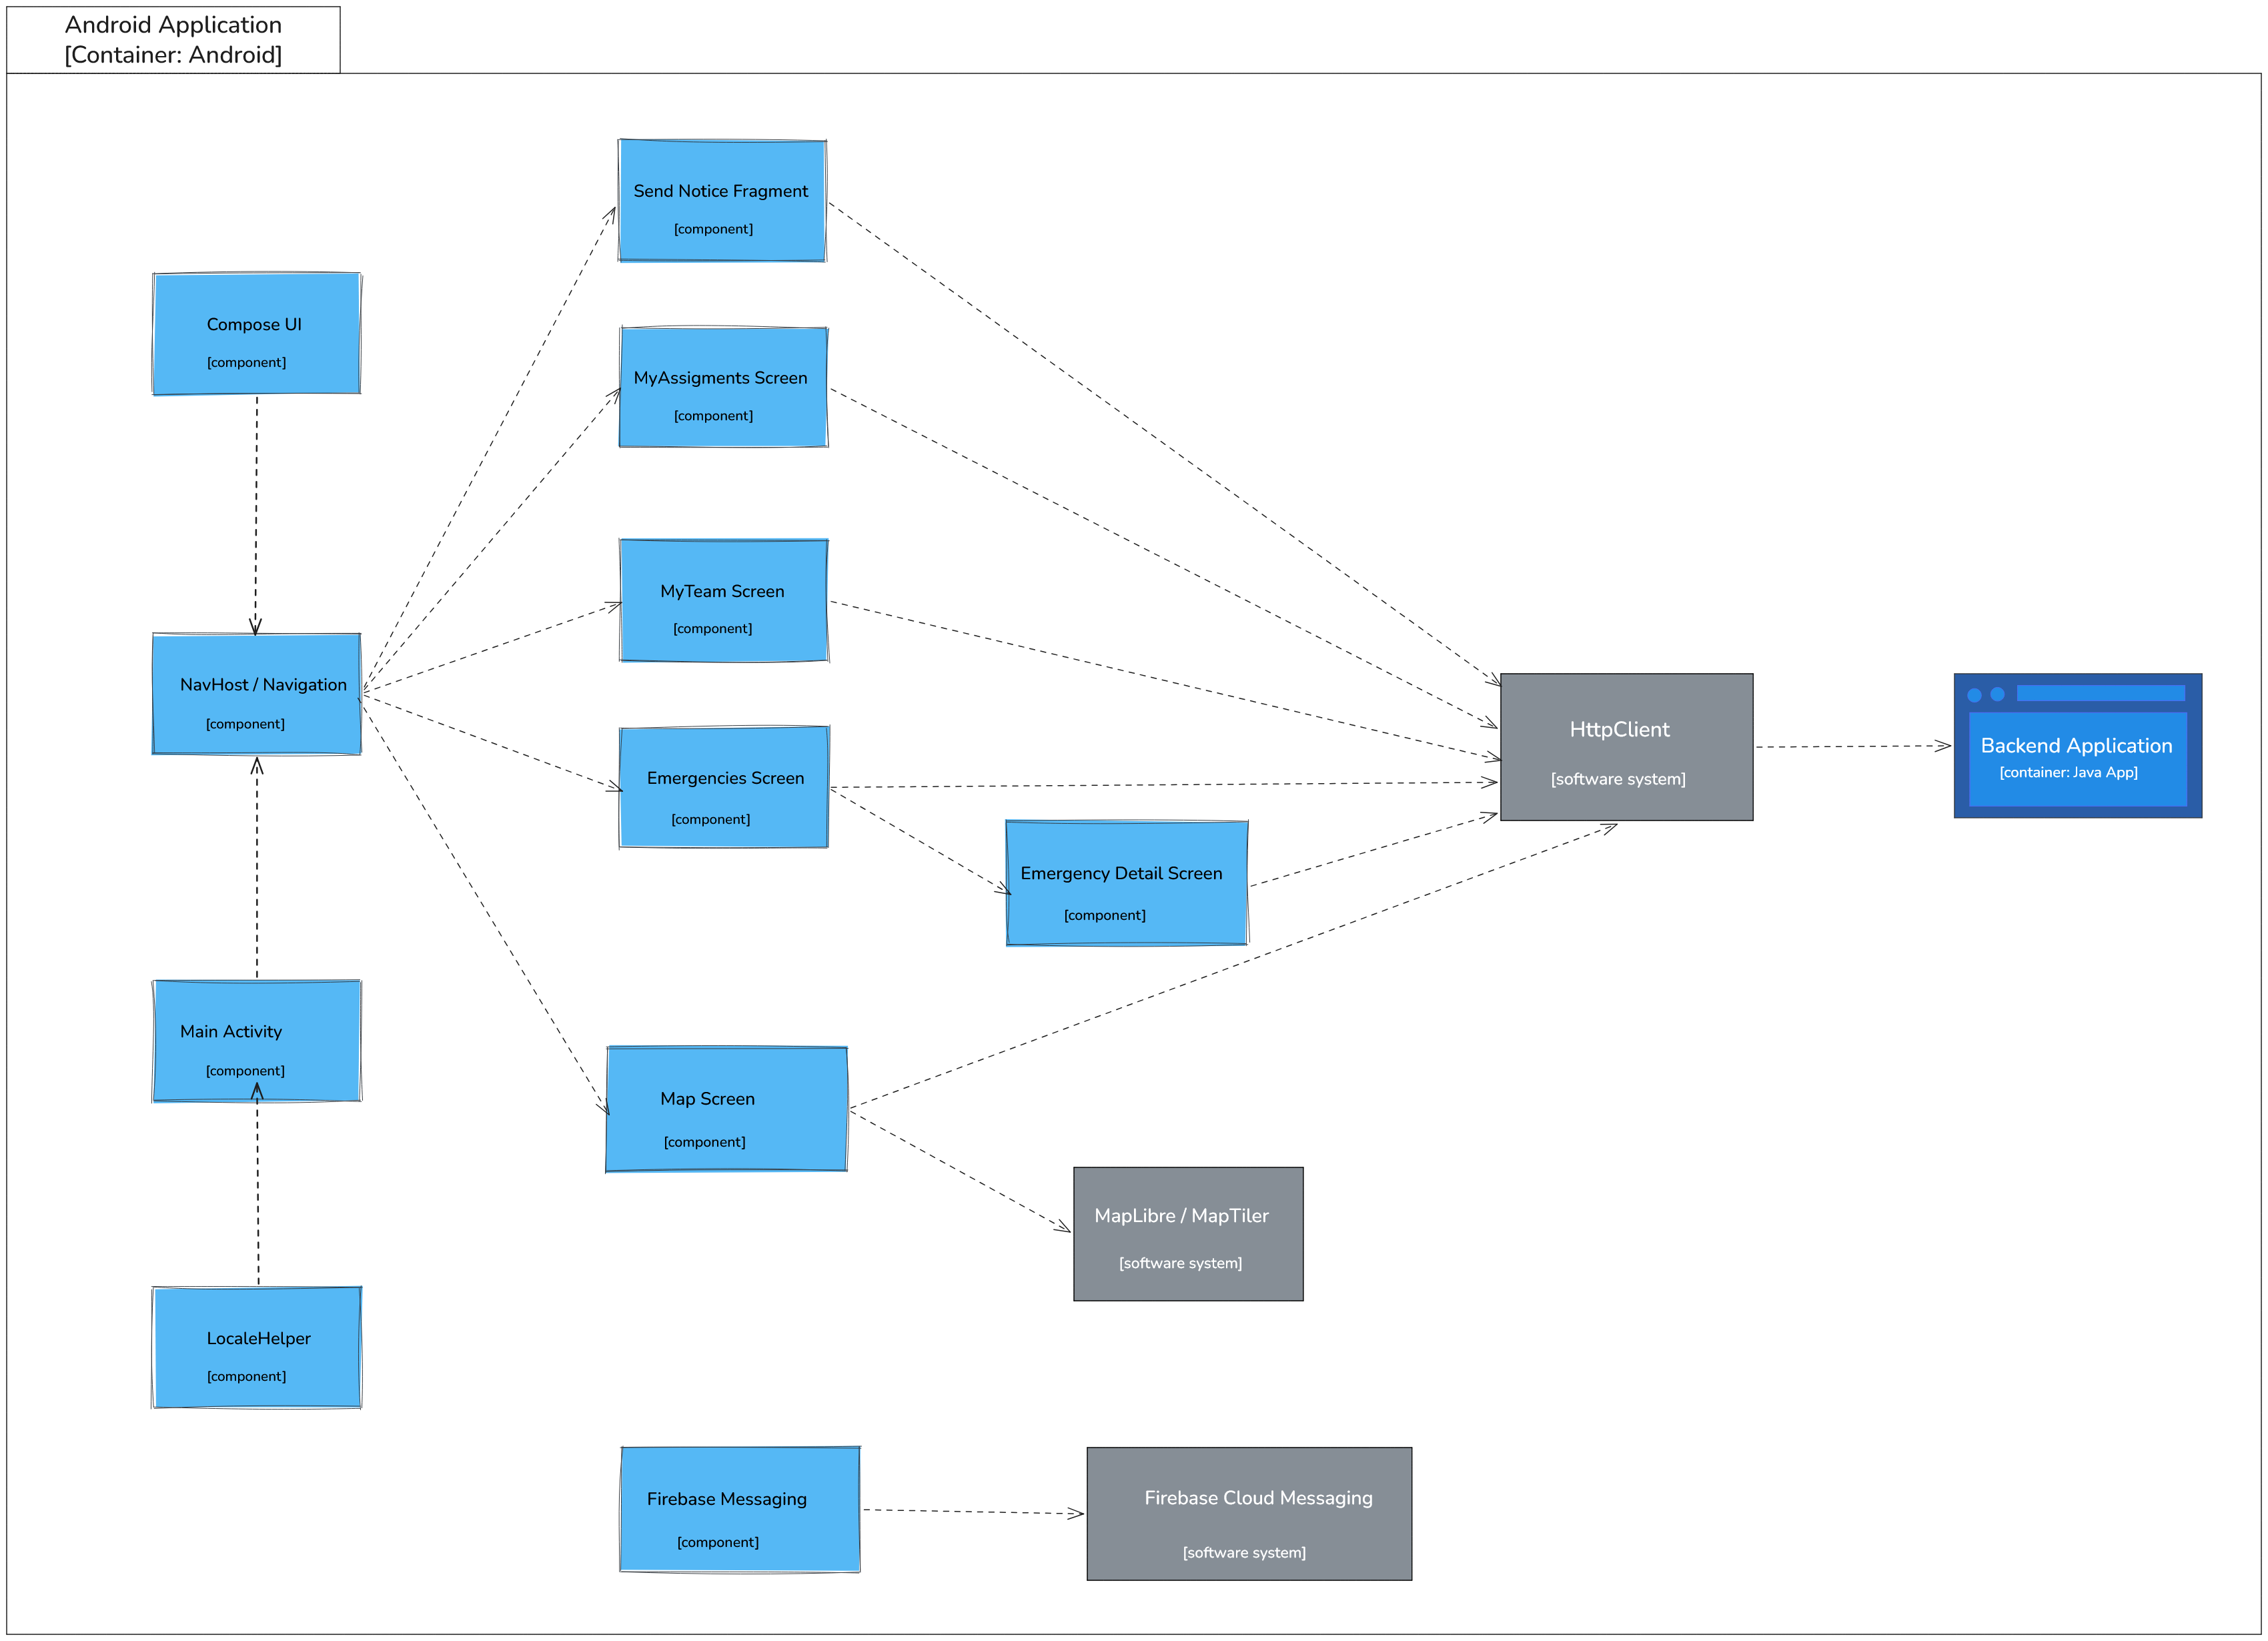
\includegraphics[width=\textwidth]{imaxes/c4/c4_container_android.png}
  \caption{Diagrama C4 de contenedores de Android}
  \label{fig:c4-container-android}
\end{figure}

En la figura \ref{fig:c4-container-android} se muestra la aplicación Android como un contenedor que agrupa navegación, pantallas Compose, accesos puntuales basados en Activities y Fragments, acceso a red, localización, Firebase Messaging e integración con mapas. La vista deja claro que el móvil consume el backend y complementa la interacción con notificaciones y servicios externos.

\subsection{Capa de acceso al servicio}

Las peticiones se realizan mediante \textit{HttpClient}, que resuelve GET y POST contra varios hosts y añade la cabecera de autorización cuando existe sesión. Este diseño simplifica la reutilización y evita repetir código de conexión en cada pantalla.

Las pantallas consumen los mismos recursos del backend que el frontend web, por lo que la capa de acceso se limita a transformar el JSON recibido en estructuras manejables desde Kotlin. En la práctica, esta capa actúa como un adaptador entre el backend y la UI móvil: abstrae la construcción de URLs, reutiliza el token almacenado en preferencias compartidas y centraliza la lógica de reintento sobre varios hosts locales. Esto evita que cada pantalla tenga que implementar su propia comunicación y hace que el acceso a datos sea homogéneo en toda la aplicación.


Como se puede observar en el siguiente diagrama de secuencia \ref{fig:secuencia-httpclient}, cuando el usuario quiere obtener información sobre las emergencias y los recursos asignados a dicha emergencia, el sistema Android realiza una serie de llamadas a la capa REST del backend, a través de la capa de acceso a servicios, para obtener la información necesaria y mostrarla en la interfaz de usuario. El proceso comienza con la pantalla de emergencias, que solicita al backend la lista de emergencias activas. Una vez que el usuario selecciona una emergencia específica, la aplicación realiza una nueva llamada para obtener el detalle de esa emergencia, incluyendo su localización y los cuadrantes asociados. Si la emergencia tiene localización por punto, se realiza una consulta adicional para determinar el cuadrante correspondiente. Finalmente, se recuperan las asignaciones vinculadas a ese cuadrante para mostrar los recursos desplegados en esa emergencia. Este flujo de llamadas garantiza que la información mostrada al usuario esté siempre actualizada y refleje el estado real del sistema gestionado por el backend.


\begin{figure}[H]
  \centering
  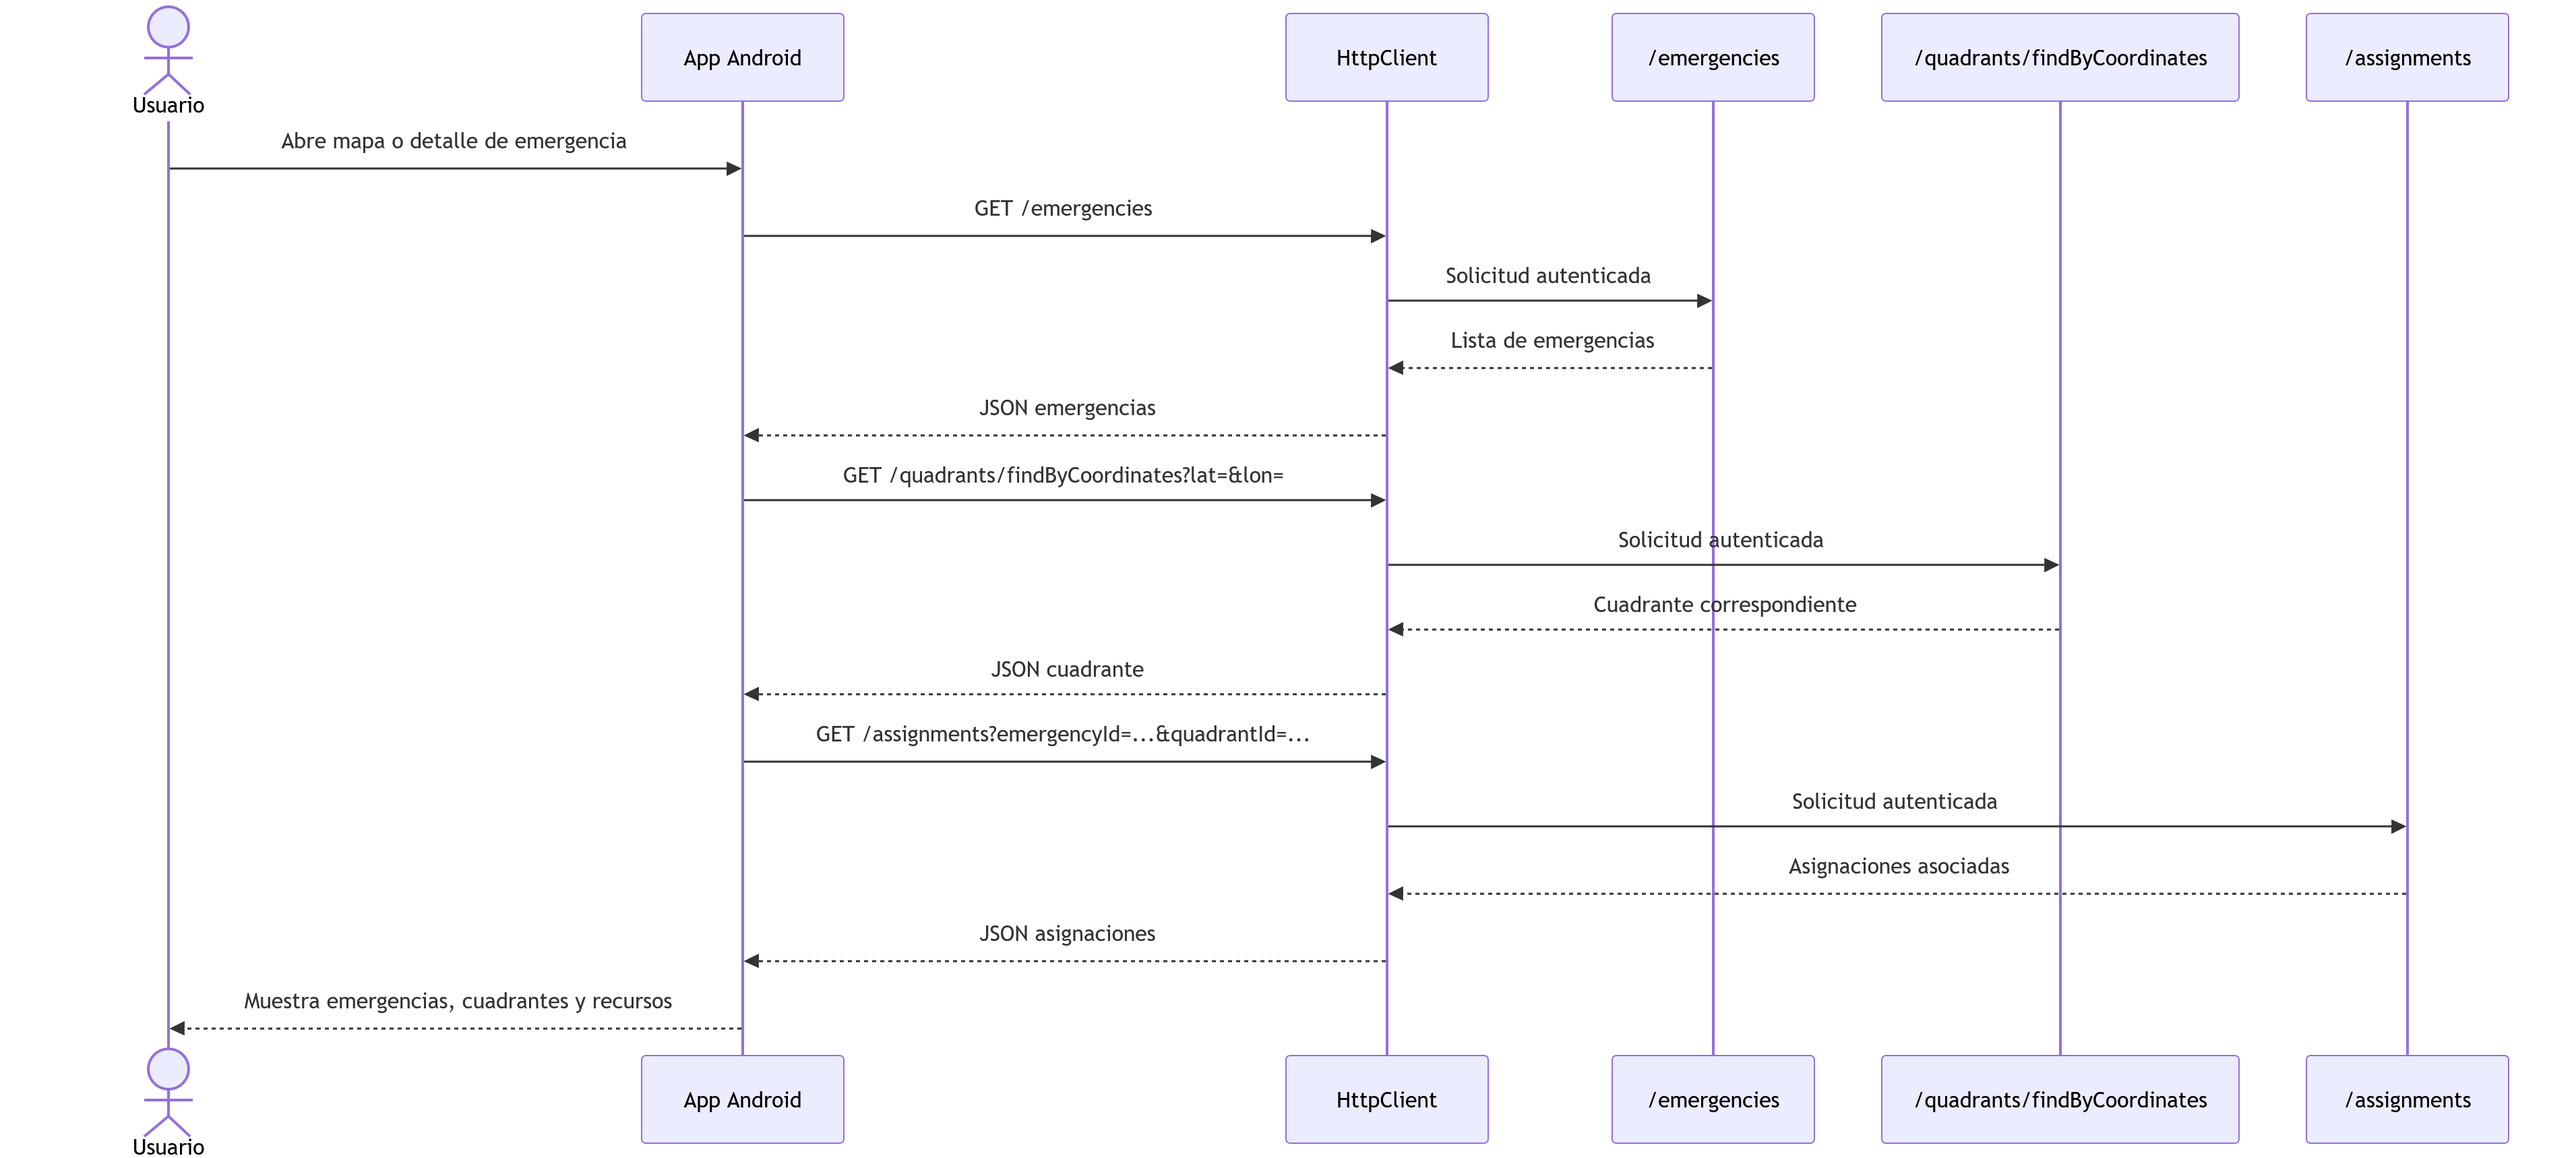
\includegraphics[width=\textwidth]{imaxes/diagrama-secuencia-httpclient.png}
  \caption{Diagrama de secuencia de comunicación entre la capa de acceso a servicios y el backend}
  \label{fig:secuencia-httpclient}
\end{figure}



\subsection{Capa de componentes de interfaz}

La pantalla principal se define en \textit{MainActivity} y su navegación agrupa cuatro bloques principales: mapa, avisos, equipo y gestión. Dentro del contenedor principal, \textit{Scaffold} organiza la barra superior y el menú lateral, mientras que el \textit{NavHost} decide qué pantalla se muestra en cada momento. Esa estructura permite navegar de forma coherente entre las distintas funcionalidades sin abandonar la actividad principal.

\textit{MapScreen} usa MapLibre para mostrar cuadrantes activos y emergencias, y actúa como una vista geoespacial central dentro de la aplicación. \textit{EmergenciesScreen} lista emergencias filtrables y permite abrir su detalle. \textit{EmergencyDetailScreen} muestra la información de la emergencia, los cuadrantes vinculados y los recursos asociados, por lo que concentra buena parte de la navegación operativa. Cuando la emergencia está localizada por coordenadas, la pantalla además calcula el cuadrante correspondiente y consulta las asignaciones asociadas para ofrecer una visión más precisa del despliegue.

La vista \textit{OrganizationsScreen} permite consultar organizaciones y aplicar filtros por nombre o tipo. \textit{ProfileScreen} muestra los datos del usuario y ofrece cambio de idioma y cierre de sesión. \textit{MyTeamScreen} presenta el equipo del usuario, sus miembros y el acceso a las asignaciones activas. \textit{MyAssignmentsScreen} lista las asignaciones pendientes y permite aceptarlas desde el propio dispositivo cuando el usuario dispone de permisos. Este flujo se apoya en la información almacenada localmente y en la sincronización con el backend para mantener el estado del recurso actualizado.

En esta capa también destaca el comportamiento del menú lateral: si el usuario no ha iniciado sesión se muestra un acceso directo al inicio de sesión, mientras que si existe sesión activa se muestran el avatar, el nombre y los bloques de navegación disponibles según el rol. Además, el menú calcula el número de asignaciones pendientes y lo muestra como indicador, ofreciendo una visión rápida del trabajo pendiente sin entrar en cada pantalla.

El envío de avisos se gestiona en \textit{SendNoticeFragment}, donde se combinan captura de imagen, obtención de localización y envío al backend. Esa pantalla refleja bien el objetivo de la app móvil: acercar al usuario acciones directas y relacionadas con su situación física. 

Otro aspecto relevante de la interfaz Android es la gestión de notificaciones push. Para explicar este proceso se ha incluido un diagrama de secuencia \ref{fig:secuencia-fcm} que resume el flujo desde que el backend envía una notificación FCM hasta que el usuario interactúa con ella. El proceso comienza con el backend generando una asignación y el \textit{AssignmentService} enviando una notificación FCM al dispositivo asociado al usuario asignado. La aplicación Android recibe esa notificación a través de \textit{AppFirebaseMessagingService}, que crea una notificación del sistema con el contenido recibido. Cuando el usuario pulsa sobre la notificación, la aplicación redirige al usuario a la pantalla de detalle de la emergencia asociada a esa asignación, permitiéndole consultar la información relevante y aceptar la asignación si lo desea. Este flujo garantiza que los usuarios estén informados en tiempo real sobre las asignaciones que les afectan y puedan reaccionar de forma inmediata desde su dispositivo móvil.

\begin{figure}[H]
  \centering
  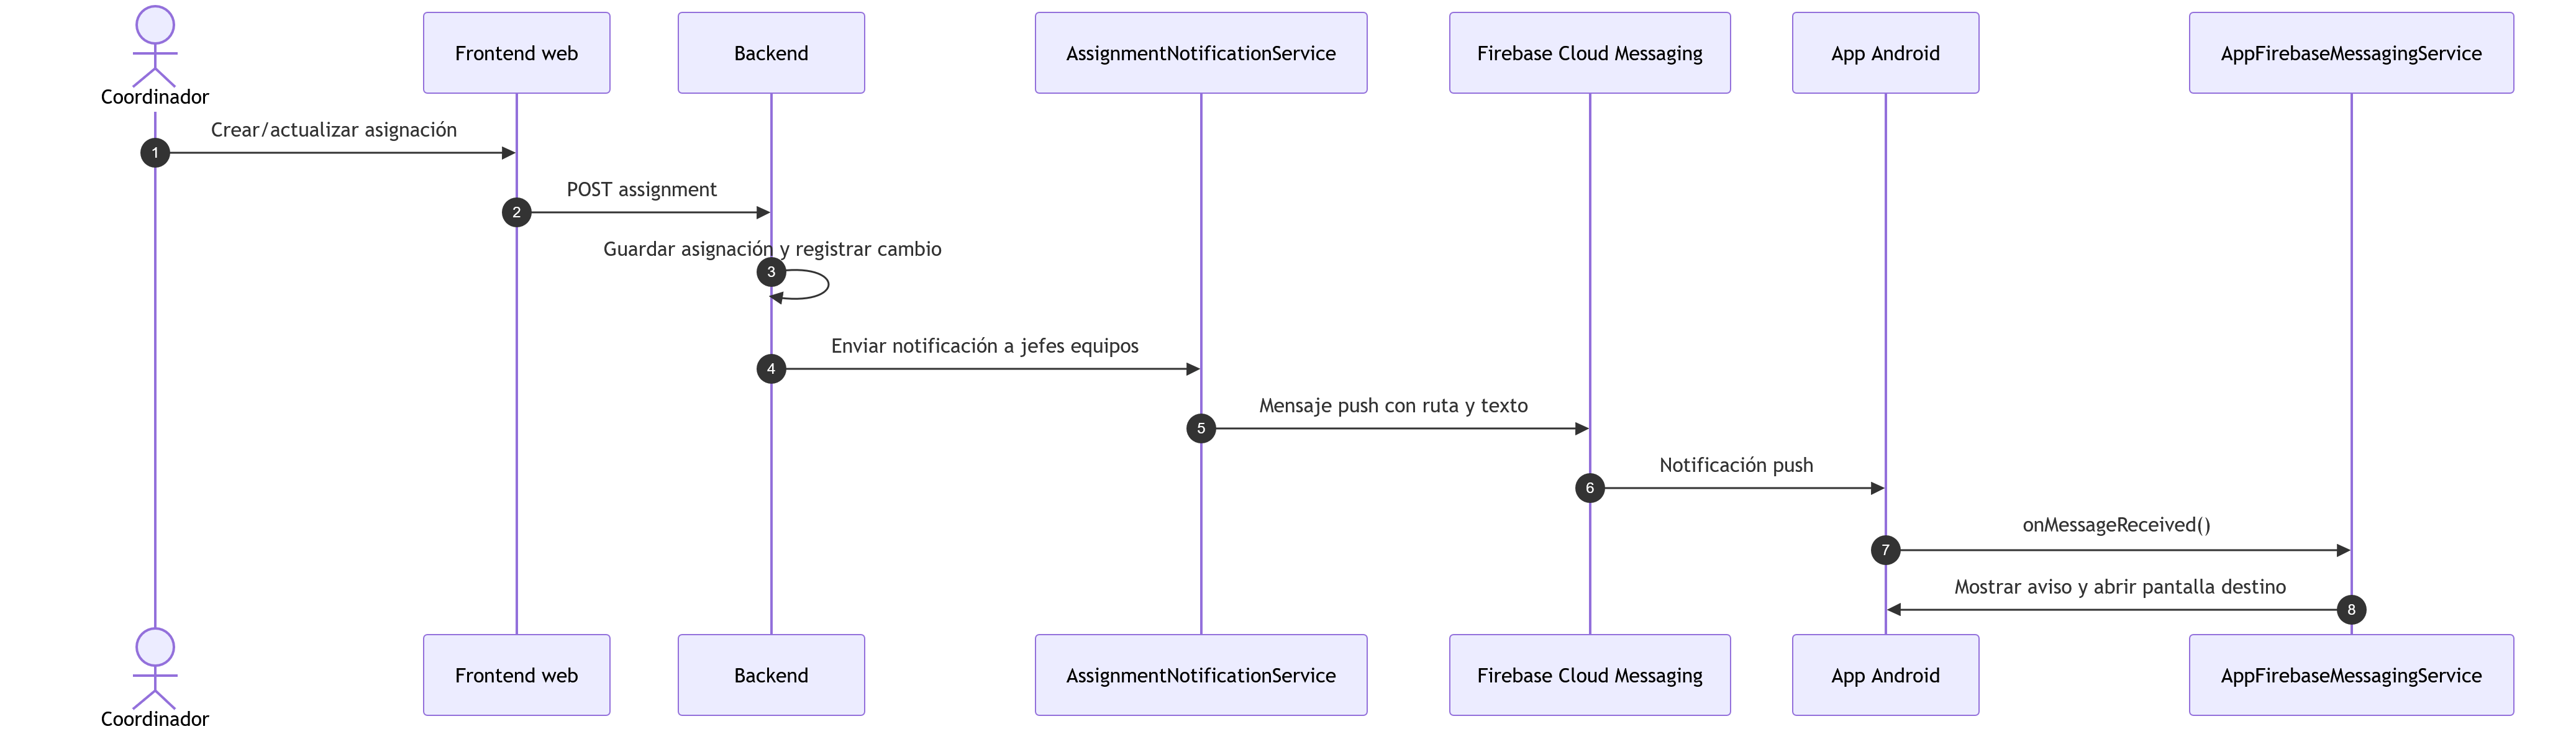
\includegraphics[width=\textwidth]{imaxes/diagrama-secuencia-fcm.png}
  \caption{Diagrama de secuencia de notificaciones FCM en Android}
  \label{fig:secuencia-fcm}
\end{figure}


\subsection{Internacionalización y librerías externas}

La internacionalización móvil se apoya en recursos de cadenas y en un \textit{helper} propio para persistir el idioma activo. La aplicación también integra Firebase Messaging, MapLibre, Glide y Proj4J, además de utilidades para transformar coordenadas entre sistemas geográficos y proyectados.
